% Manuscript draft — target: Journal of Neural Engineering (IOP). Generic article class for drafting;
% switch to iopart at submission. Every number in Results/Discussion is generated by NB07 from the
% committed raw runs in reports/ (see paper/generated/); none is typed by hand.
\documentclass[11pt]{article}
\usepackage[margin=2.5cm]{geometry}
\usepackage[T1]{fontenc}
\usepackage[utf8]{inputenc}
\usepackage{lmodern,microtype,amsmath,amssymb,booktabs,graphicx,xcolor,siunitx}
\usepackage[numbers,sort&compress]{natbib}
\usepackage{tikz}
\usetikzlibrary{positioning,arrows.meta}
\usepackage[hidelinks]{hyperref}
\graphicspath{{generated/figures/}}
% generated by paper/make_numbers.py — do not edit
\newcommand{\ablPThreehybridAFivedepthOneDelta}{\ensuremath{-}0.006}
\newcommand{\ablPThreehybridAFivedepthOneHi}{+0.031}
\newcommand{\ablPThreehybridAFivedepthOneLo}{\ensuremath{-}0.042}
\newcommand{\ablPThreehybridAFivedepthOneP}{=1.000}
\newcommand{\ablPThreehybridAFivedepthThreeDelta}{+0.007}
\newcommand{\ablPThreehybridAFivedepthThreeHi}{+0.033}
\newcommand{\ablPThreehybridAFivedepthThreeLo}{\ensuremath{-}0.018}
\newcommand{\ablPThreehybridAFivedepthThreeP}{=1.000}
\newcommand{\ablPThreehybridAFourbinaryDelta}{\ensuremath{-}0.023}
\newcommand{\ablPThreehybridAFourbinaryHi}{+0.011}
\newcommand{\ablPThreehybridAFourbinaryLo}{\ensuremath{-}0.057}
\newcommand{\ablPThreehybridAFourbinaryP}{=1.000}
\newcommand{\ablPThreehybridANineunweightedDelta}{+0.014}
\newcommand{\ablPThreehybridANineunweightedHi}{+0.044}
\newcommand{\ablPThreehybridANineunweightedLo}{\ensuremath{-}0.016}
\newcommand{\ablPThreehybridANineunweightedP}{=1.000}
\newcommand{\ablPThreehybridAOneTworesidualizedDelta}{\ensuremath{-}0.044}
\newcommand{\ablPThreehybridAOneTworesidualizedHi}{+0.004}
\newcommand{\ablPThreehybridAOneTworesidualizedLo}{\ensuremath{-}0.093}
\newcommand{\ablPThreehybridAOneTworesidualizedP}{=1.000}
\newcommand{\ablPThreehybridAOnenographDelta}{\ensuremath{-}0.024}
\newcommand{\ablPThreehybridAOnenographHi}{+0.015}
\newcommand{\ablPThreehybridAOnenographLo}{\ensuremath{-}0.064}
\newcommand{\ablPThreehybridAOnenographP}{=1.000}
\newcommand{\ablPThreehybridASixgatDelta}{\ensuremath{-}0.021}
\newcommand{\ablPThreehybridASixgatHi}{+0.002}
\newcommand{\ablPThreehybridASixgatLo}{\ensuremath{-}0.044}
\newcommand{\ablPThreehybridASixgatP}{=1.000}
\newcommand{\ablPThreehybridAThreefullDelta}{\ensuremath{-}0.032}
\newcommand{\ablPThreehybridAThreefullHi}{+0.005}
\newcommand{\ablPThreehybridAThreefullLo}{\ensuremath{-}0.068}
\newcommand{\ablPThreehybridAThreefullP}{=1.000}
\newcommand{\ablPThreehybridAThreekSixDelta}{+0.000}
\newcommand{\ablPThreehybridAThreekSixHi}{+0.032}
\newcommand{\ablPThreehybridAThreekSixLo}{\ensuremath{-}0.031}
\newcommand{\ablPThreehybridAThreekSixP}{=1.000}
\newcommand{\ablPThreehybridAThreekThreeDelta}{\ensuremath{-}0.009}
\newcommand{\ablPThreehybridAThreekThreeHi}{+0.007}
\newcommand{\ablPThreehybridAThreekThreeLo}{\ensuremath{-}0.026}
\newcommand{\ablPThreehybridAThreekThreeP}{=1.000}
\newcommand{\ablPThreehybridATworandomgraphDelta}{\ensuremath{-}0.018}
\newcommand{\ablPThreehybridATworandomgraphHi}{+0.013}
\newcommand{\ablPThreehybridATworandomgraphLo}{\ensuremath{-}0.049}
\newcommand{\ablPThreehybridATworandomgraphP}{=1.000}
\newcommand{\ablPThreehybridRQSevenplusPSevenDelta}{+0.005}
\newcommand{\ablPThreehybridRQSevenplusPSevenHi}{+0.038}
\newcommand{\ablPThreehybridRQSevenplusPSevenLo}{\ensuremath{-}0.028}
\newcommand{\ablPThreehybridRQSevenplusPSevenP}{=1.000}
\newcommand{\ablPThreehybridRQSevenpsweedgeDelta}{\ensuremath{-}0.011}
\newcommand{\ablPThreehybridRQSevenpsweedgeHi}{+0.022}
\newcommand{\ablPThreehybridRQSevenpsweedgeLo}{\ensuremath{-}0.044}
\newcommand{\ablPThreehybridRQSevenpsweedgeP}{=1.000}
\newcommand{\ablPThreespatialAFivedepthOneDelta}{\ensuremath{-}0.026}
\newcommand{\ablPThreespatialAFivedepthOneHi}{+0.020}
\newcommand{\ablPThreespatialAFivedepthOneLo}{\ensuremath{-}0.073}
\newcommand{\ablPThreespatialAFivedepthOneP}{=1.000}
\newcommand{\ablPThreespatialAFivedepthThreeDelta}{\ensuremath{-}0.010}
\newcommand{\ablPThreespatialAFivedepthThreeHi}{+0.022}
\newcommand{\ablPThreespatialAFivedepthThreeLo}{\ensuremath{-}0.042}
\newcommand{\ablPThreespatialAFivedepthThreeP}{=1.000}
\newcommand{\ablPThreespatialAFourbinaryDelta}{\ensuremath{-}0.006}
\newcommand{\ablPThreespatialAFourbinaryHi}{+0.008}
\newcommand{\ablPThreespatialAFourbinaryLo}{\ensuremath{-}0.020}
\newcommand{\ablPThreespatialAFourbinaryP}{=1.000}
\newcommand{\ablPThreespatialANineunweightedDelta}{+0.007}
\newcommand{\ablPThreespatialANineunweightedHi}{+0.044}
\newcommand{\ablPThreespatialANineunweightedLo}{\ensuremath{-}0.030}
\newcommand{\ablPThreespatialANineunweightedP}{=1.000}
\newcommand{\ablPThreespatialAOneTworesidualizedDelta}{\ensuremath{-}0.046}
\newcommand{\ablPThreespatialAOneTworesidualizedHi}{\ensuremath{-}0.003}
\newcommand{\ablPThreespatialAOneTworesidualizedLo}{\ensuremath{-}0.089}
\newcommand{\ablPThreespatialAOneTworesidualizedP}{=1.000}
\newcommand{\ablPThreespatialAOnenographDelta}{\ensuremath{-}0.043}
\newcommand{\ablPThreespatialAOnenographHi}{+0.003}
\newcommand{\ablPThreespatialAOnenographLo}{\ensuremath{-}0.088}
\newcommand{\ablPThreespatialAOnenographP}{=1.000}
\newcommand{\ablPThreespatialASixgatDelta}{\ensuremath{-}0.022}
\newcommand{\ablPThreespatialASixgatHi}{+0.025}
\newcommand{\ablPThreespatialASixgatLo}{\ensuremath{-}0.069}
\newcommand{\ablPThreespatialASixgatP}{=1.000}
\newcommand{\ablPThreespatialAThreefullDelta}{\ensuremath{-}0.066}
\newcommand{\ablPThreespatialAThreefullHi}{\ensuremath{-}0.020}
\newcommand{\ablPThreespatialAThreefullLo}{\ensuremath{-}0.113}
\newcommand{\ablPThreespatialAThreefullP}{=1.000}
\newcommand{\ablPThreespatialAThreekSixDelta}{\ensuremath{-}0.009}
\newcommand{\ablPThreespatialAThreekSixHi}{+0.015}
\newcommand{\ablPThreespatialAThreekSixLo}{\ensuremath{-}0.033}
\newcommand{\ablPThreespatialAThreekSixP}{=1.000}
\newcommand{\ablPThreespatialAThreekThreeDelta}{\ensuremath{-}0.022}
\newcommand{\ablPThreespatialAThreekThreeHi}{+0.004}
\newcommand{\ablPThreespatialAThreekThreeLo}{\ensuremath{-}0.047}
\newcommand{\ablPThreespatialAThreekThreeP}{=1.000}
\newcommand{\ablPThreespatialATworandomgraphDelta}{\ensuremath{-}0.037}
\newcommand{\ablPThreespatialATworandomgraphHi}{+0.002}
\newcommand{\ablPThreespatialATworandomgraphLo}{\ensuremath{-}0.075}
\newcommand{\ablPThreespatialATworandomgraphP}{=1.000}
\newcommand{\ablPThreespatialRQSevenplusPSevenDelta}{\ensuremath{-}0.024}
\newcommand{\ablPThreespatialRQSevenplusPSevenHi}{+0.011}
\newcommand{\ablPThreespatialRQSevenplusPSevenLo}{\ensuremath{-}0.059}
\newcommand{\ablPThreespatialRQSevenplusPSevenP}{=1.000}
\newcommand{\ablPThreespatialRQSevenpsweedgeDelta}{\ensuremath{-}0.029}
\newcommand{\ablPThreespatialRQSevenpsweedgeHi}{+0.007}
\newcommand{\ablPThreespatialRQSevenpsweedgeLo}{\ensuremath{-}0.065}
\newcommand{\ablPThreespatialRQSevenpsweedgeP}{=1.000}
\newcommand{\anovaEdgeDfOne}{2}
\newcommand{\anovaEdgeDfTwo}{48}
\newcommand{\anovaEdgeEta}{0.14}
\newcommand{\anovaEdgeF}{4.03}
\newcommand{\anovaEdgeP}{=0.026}
\newcommand{\anovaInterDfOne}{12}
\newcommand{\anovaInterDfTwo}{288}
\newcommand{\anovaInterEta}{0.06}
\newcommand{\anovaInterF}{1.43}
\newcommand{\anovaInterP}{=0.194}
\newcommand{\anovaRepDfOne}{6}
\newcommand{\anovaRepDfTwo}{144}
\newcommand{\anovaRepEta}{0.33}
\newcommand{\anovaRepF}{11.83}
\newcommand{\anovaRepP}{<0.001}
\newcommand{\bestAcc}{0.614}
\newcommand{\bestAuc}{0.749}
\newcommand{\bestBalAcc}{0.594}
\newcommand{\bestBrier}{0.558}
\newcommand{\bestCell}{P3\,$\times$\,spatial}
\newcommand{\bestEce}{0.265}
\newcommand{\bestFOne}{0.586}
\newcommand{\bestFOneCiHi}{0.628}
\newcommand{\bestFOneCiLo}{0.538}
\newcommand{\bestFOneSd}{0.112}
\newcommand{\bestKappa}{0.409}
\newcommand{\bestSensAD}{0.642}
\newcommand{\bestSensCN}{0.771}
\newcommand{\bestSensFTD}{0.368}
\newcommand{\bestSpecAD}{0.775}
\newcommand{\bestSpecCN}{0.786}
\newcommand{\bestSpecFTD}{0.852}
\newcommand{\cdValue}{6.26}
\newcommand{\cellPFivefunctional}{0.504}
\newcommand{\cellPFivehybrid}{0.470}
\newcommand{\cellPFivespatial}{0.494}
\newcommand{\cellPFourfunctional}{0.418}
\newcommand{\cellPFourhybrid}{0.430}
\newcommand{\cellPFourspatial}{0.456}
\newcommand{\cellPOnefunctional}{0.551}
\newcommand{\cellPOnehybrid}{0.545}
\newcommand{\cellPOnespatial}{0.560}
\newcommand{\cellPSevenfunctional}{0.444}
\newcommand{\cellPSevenhybrid}{0.445}
\newcommand{\cellPSevenspatial}{0.454}
\newcommand{\cellPSixfunctional}{0.556}
\newcommand{\cellPSixhybrid}{0.532}
\newcommand{\cellPSixspatial}{0.540}
\newcommand{\cellPThreefunctional}{0.553}
\newcommand{\cellPThreehybrid}{0.568}
\newcommand{\cellPThreespatial}{0.586}
\newcommand{\cellPTwofunctional}{0.455}
\newcommand{\cellPTwohybrid}{0.451}
\newcommand{\cellPTwospatial}{0.454}
\newcommand{\chanceFOne}{0.302}
\newcommand{\cpuHoursGrid}{2.4}
\newcommand{\demoFOne}{0.411}
\newcommand{\edgefunctional}{0.497}
\newcommand{\edgehybrid}{0.492}
\newcommand{\edgespatial}{0.506}
\newcommand{\friedmanP}{<0.001}
\newcommand{\gvcPFourClassical}{0.487}
\newcommand{\gvcPFourDelta}{\ensuremath{-}0.031}
\newcommand{\gvcPFourP}{=1.000}
\newcommand{\gvcPOneClassical}{0.588}
\newcommand{\gvcPOneDelta}{\ensuremath{-}0.028}
\newcommand{\gvcPOneP}{=1.000}
\newcommand{\gvcPSevenClassical}{0.502}
\newcommand{\gvcPSevenDelta}{\ensuremath{-}0.048}
\newcommand{\gvcPSevenP}{=1.000}
\newcommand{\gvcPSixClassical}{0.579}
\newcommand{\gvcPSixDelta}{\ensuremath{-}0.023}
\newcommand{\gvcPSixP}{=1.000}
\newcommand{\gvcPThreeClassical}{0.581}
\newcommand{\gvcPThreeDelta}{+0.005}
\newcommand{\gvcPThreeP}{=1.000}
\newcommand{\gvcPTwoClassical}{0.435}
\newcommand{\gvcPTwoDelta}{+0.020}
\newcommand{\gvcPTwoP}{=1.000}
\newcommand{\icaExcludedMean}{2.4}
\newcommand{\leakPThreehybridCorrectSubj}{0.568}
\newcommand{\leakPThreehybridInflation}{0.262}
\newcommand{\leakPThreehybridLeakySubj}{0.974}
\newcommand{\leakPThreehybridLeakyWin}{0.830}
\newcommand{\leakPThreespatialCorrectSubj}{0.586}
\newcommand{\leakPThreespatialInflation}{0.256}
\newcommand{\leakPThreespatialLeakySubj}{0.988}
\newcommand{\leakPThreespatialLeakyWin}{0.842}
\newcommand{\nAblRuns}{1,700}
\newcommand{\nMainRuns}{525}
\newcommand{\nPairs}{21}
\newcommand{\nPairsNbSig}{0}
\newcommand{\nPairsWilcoxonSig}{9}
\newcommand{\nWindows}{7,013}
\newcommand{\pThreeFourD}{1.50}
\newcommand{\pThreeFourDiff}{0.135}
\newcommand{\pThreeFourNbP}{=0.216}
\newcommand{\pThreeFourWilP}{<0.001}
\newcommand{\permPThreespatialN}{200}
\newcommand{\permPThreespatialNullMax}{0.474}
\newcommand{\permPThreespatialNullMean}{0.313}
\newcommand{\permPThreespatialObs}{0.575}
\newcommand{\permPThreespatialP}{0.005}
\newcommand{\psweAdjADHi}{5.57}
\newcommand{\psweAdjADLo}{1.58}
\newcommand{\psweAdjADP}{<0.001}
\newcommand{\psweAdjADRR}{2.96}
\newcommand{\psweAdjFTDHi}{4.15}
\newcommand{\psweAdjFTDLo}{1.03}
\newcommand{\psweAdjFTDP}{=0.041}
\newcommand{\psweAdjFTDRR}{2.07}
\newcommand{\psweAdjSlowADHi}{0.75}
\newcommand{\psweAdjSlowADLo}{0.33}
\newcommand{\psweAdjSlowADP}{<0.001}
\newcommand{\psweAdjSlowADRR}{0.50}
\newcommand{\psweAdjSlowFTDHi}{1.00}
\newcommand{\psweAdjSlowFTDLo}{0.45}
\newcommand{\psweAdjSlowFTDP}{=0.051}
\newcommand{\psweAdjSlowFTDRR}{0.67}
\newcommand{\psweKwP}{=0.041}
\newcommand{\psweMmseP}{=0.095}
\newcommand{\psweMmseRho}{\ensuremath{-}0.22}
\newcommand{\psweRateAD}{1.34}
\newcommand{\psweRateCN}{0.22}
\newcommand{\psweRateFTD}{0.41}
\newcommand{\psweSlowPartial}{0.87}
\newcommand{\psweSlowRho}{0.88}
\newcommand{\reldropOnepFiveAdjADHi}{1.02}
\newcommand{\reldropOnepFiveAdjADLo}{0.44}
\newcommand{\reldropOnepFiveAdjADP}{=0.060}
\newcommand{\reldropOnepFiveAdjADRR}{0.67}
\newcommand{\reldropOnepFiveAdjBgADHi}{1.33}
\newcommand{\reldropOnepFiveAdjBgADLo}{0.55}
\newcommand{\reldropOnepFiveAdjBgADP}{=0.478}
\newcommand{\reldropOnepFiveAdjBgADRR}{0.85}
\newcommand{\reldropOnepFiveAdjBgFTDHi}{1.37}
\newcommand{\reldropOnepFiveAdjBgFTDLo}{0.53}
\newcommand{\reldropOnepFiveAdjBgFTDP}{=0.505}
\newcommand{\reldropOnepFiveAdjBgFTDRR}{0.85}
\newcommand{\reldropOnepFiveAdjFTDHi}{1.35}
\newcommand{\reldropOnepFiveAdjFTDLo}{0.50}
\newcommand{\reldropOnepFiveAdjFTDP}{=0.431}
\newcommand{\reldropOnepFiveAdjFTDRR}{0.82}
\newcommand{\reldropOnepFiveMmseRho}{0.03}
\newcommand{\reldropOnepFiveSlowRho}{\ensuremath{-}0.08}
\newcommand{\reldropThreeAdjADHi}{0.75}
\newcommand{\reldropThreeAdjADLo}{0.25}
\newcommand{\reldropThreeAdjADP}{=0.003}
\newcommand{\reldropThreeAdjADRR}{0.43}
\newcommand{\reldropThreeAdjBgADHi}{1.20}
\newcommand{\reldropThreeAdjBgADLo}{0.38}
\newcommand{\reldropThreeAdjBgADP}{=0.179}
\newcommand{\reldropThreeAdjBgADRR}{0.67}
\newcommand{\reldropThreeAdjBgFTDHi}{1.01}
\newcommand{\reldropThreeAdjBgFTDLo}{0.29}
\newcommand{\reldropThreeAdjBgFTDP}{=0.053}
\newcommand{\reldropThreeAdjBgFTDRR}{0.54}
\newcommand{\reldropThreeAdjFTDHi}{1.09}
\newcommand{\reldropThreeAdjFTDLo}{0.29}
\newcommand{\reldropThreeAdjFTDP}{=0.088}
\newcommand{\reldropThreeAdjFTDRR}{0.56}
\newcommand{\reldropThreeMmseRho}{0.07}
\newcommand{\reldropThreeSlowRho}{\ensuremath{-}0.24}
\newcommand{\reldropTwoAdjADHi}{0.89}
\newcommand{\reldropTwoAdjADLo}{0.35}
\newcommand{\reldropTwoAdjADP}{=0.014}
\newcommand{\reldropTwoAdjADRR}{0.55}
\newcommand{\reldropTwoAdjBgADHi}{1.26}
\newcommand{\reldropTwoAdjBgADLo}{0.47}
\newcommand{\reldropTwoAdjBgADP}{=0.299}
\newcommand{\reldropTwoAdjBgADRR}{0.77}
\newcommand{\reldropTwoAdjBgFTDHi}{1.20}
\newcommand{\reldropTwoAdjBgFTDLo}{0.42}
\newcommand{\reldropTwoAdjBgFTDP}{=0.198}
\newcommand{\reldropTwoAdjBgFTDRR}{0.71}
\newcommand{\reldropTwoAdjFTDHi}{1.23}
\newcommand{\reldropTwoAdjFTDLo}{0.40}
\newcommand{\reldropTwoAdjFTDP}{=0.213}
\newcommand{\reldropTwoAdjFTDRR}{0.70}
\newcommand{\reldropTwoMmseRho}{0.04}
\newcommand{\reldropTwoSlowRho}{\ensuremath{-}0.15}
\newcommand{\relmadThreeAdjADHi}{0.40}
\newcommand{\relmadThreeAdjADLo}{0.07}
\newcommand{\relmadThreeAdjADP}{<0.001}
\newcommand{\relmadThreeAdjADRR}{0.17}
\newcommand{\relmadThreeAdjBgADHi}{0.85}
\newcommand{\relmadThreeAdjBgADLo}{0.14}
\newcommand{\relmadThreeAdjBgADP}{=0.020}
\newcommand{\relmadThreeAdjBgADRR}{0.35}
\newcommand{\relmadThreeAdjBgFTDHi}{0.75}
\newcommand{\relmadThreeAdjBgFTDLo}{0.13}
\newcommand{\relmadThreeAdjBgFTDP}{=0.010}
\newcommand{\relmadThreeAdjBgFTDRR}{0.31}
\newcommand{\relmadThreeAdjFTDHi}{0.71}
\newcommand{\relmadThreeAdjFTDLo}{0.10}
\newcommand{\relmadThreeAdjFTDP}{=0.008}
\newcommand{\relmadThreeAdjFTDRR}{0.27}
\newcommand{\relmadThreeMmseRho}{0.14}
\newcommand{\relmadThreeSlowRho}{\ensuremath{-}0.57}
\newcommand{\relmadTwoAdjADHi}{0.46}
\newcommand{\relmadTwoAdjADLo}{0.13}
\newcommand{\relmadTwoAdjADP}{<0.001}
\newcommand{\relmadTwoAdjADRR}{0.24}
\newcommand{\relmadTwoAdjBgADHi}{0.84}
\newcommand{\relmadTwoAdjBgADLo}{0.22}
\newcommand{\relmadTwoAdjBgADP}{=0.014}
\newcommand{\relmadTwoAdjBgADRR}{0.43}
\newcommand{\relmadTwoAdjBgFTDHi}{0.68}
\newcommand{\relmadTwoAdjBgFTDLo}{0.18}
\newcommand{\relmadTwoAdjBgFTDP}{=0.002}
\newcommand{\relmadTwoAdjBgFTDRR}{0.35}
\newcommand{\relmadTwoAdjFTDHi}{0.69}
\newcommand{\relmadTwoAdjFTDLo}{0.16}
\newcommand{\relmadTwoAdjFTDP}{=0.003}
\newcommand{\relmadTwoAdjFTDRR}{0.33}
\newcommand{\relmadTwoMmseRho}{0.11}
\newcommand{\relmadTwoSlowRho}{\ensuremath{-}0.54}
\newcommand{\repPFive}{0.489}
\newcommand{\repPFour}{0.434}
\newcommand{\repPOne}{0.552}
\newcommand{\repPSeven}{0.448}
\newcommand{\repPSix}{0.543}
\newcommand{\repPThree}{0.569}
\newcommand{\repPTwo}{0.453}
\newcommand{\thetaAlphaAD}{1.57}
\newcommand{\thetaAlphaCN}{0.28}
\newcommand{\thetaAlphaFTD}{0.68}
   % every result quoted in the text (paper/make_numbers.py)
\makeatletter
\newcommand{\inputtab}[1]{\@@input #1 }   % primitive \input: safe inside tabular
\makeatother

\title{Representation, Topology, and a Blood--Brain-Barrier-Associated Slow-Wave Marker:\\
A Controlled Graph Neural Network Study of EEG in Alzheimer's Disease and Frontotemporal Dementia}
\author{Devguru\\ Indian Institute of Information Technology, Nagpur\\ \texttt{bt23csd060@iiitn.ac.in}}
\date{Draft --- \today}

\begin{document}
\maketitle

\begin{abstract}
\textit{Objective.} EEG-based classification of Alzheimer's disease (AD) and frontotemporal dementia
(FTD) on the same public dataset reports accuracies from 80\% to 99\%, but studies change the signal
representation, graph construction, model and evaluation protocol at once. We isolated these factors
and tested a blood--brain-barrier (BBB)-associated EEG marker.
\textit{Approach.} Using OpenNeuro ds004504 (36 AD, 23 FTD, 29 controls), we crossed seven node-feature
representations with three graph constructions under one fixed two-layer graph convolutional network,
evaluated on 25 frozen, paired subject-level cross-validation splits (\nMainRuns{} runs) and
re-evaluated on 25 independent confirmation splits, with non-graph baselines trained on matched
subjects, ablation and permutation runs on the confirmation splits, and a leakage experiment. We also
characterised paroxysmal slow-wave events (PSWEs), an EEG marker linked to BBB dysfunction.
\textit{Main results.} Representation had a large effect on three-class macro-F1 (partial
$\eta^2=\anovaRepEta$, replicated at \canovaRepEta{}); a small graph-construction effect
($\eta^2=\anovaEdgeEta$) did not replicate, and there was no interaction. The best configuration
(wavelet features, spatial graph) reached \confFOne{} on the independent confirmation splits (95\% CI
\confFOneCiLo{}--\confFOneCiHi{}; permutation $p=\cpermPThreespatialP$), not significantly different
from non-graph classifiers trained on the same subjects. Window-level splitting of the identical
pipeline raised it to \cleakPThreespatialLeakySubj{}. Fixed-threshold PSWEs were more frequent in AD (rate ratio
\psweAdjADRR{}) and FTD (\psweAdjFTDRR{}) than in controls, but this was explained by background slowing
($\rho=\psweSlowRho$); relative to each person's background, transient slowing events were less
frequent in dementia.
\textit{Significance.} On this benchmark the signal representation and, above all, the evaluation
protocol --- not the graph or the model --- determine reported performance, and an EEG marker of BBB
dysfunction must be defined relative to background slowing. Code, frozen folds and all raw runs are
released.

\end{abstract}

\noindent\textbf{Keywords:} EEG; graph neural network; Alzheimer's disease; frontotemporal dementia;
signal representation; functional connectivity; blood--brain barrier; paroxysmal slow-wave events;
data leakage; reproducibility

\section{Introduction}\label{sec:intro}

% TODO (author): add 2--3 current epidemiology references for this opening claim (paper_structure.md §1).
Alzheimer's disease (AD) and frontotemporal dementia (FTD) are leading causes of neurodegenerative
dementia, particularly with onset before 65, and telling them apart is clinically consequential:
they differ in prognosis, in care needs and in which disease-modifying treatments are appropriate.
Scalp electroencephalography (EEG) is attractive for this task because it is cheap, non-invasive and
available in routine care, in contrast to amyloid PET or MRI. Its physiological basis is well
established: AD is increasingly understood as a disorder of large-scale brain networks
\cite{F12}, and graph-theoretical EEG studies have shown that AD and FTD disturb those networks in
\emph{different} ways \cite{F9}, which is what makes a three-class AD/FTD/control problem
scientifically meaningful rather than merely harder.

Machine-learning work on this question has moved from spectral markers and handcrafted features with
classical classifiers \cite{F10} to convolutional networks and transformers \cite{F2,R14} and,
most recently, to graph neural networks (GNNs) that treat electrodes as nodes and inter-electrode
coupling as edges \cite{F5,F3,F4,F6,R9,R10,R12}. The public OpenNeuro dataset ds004504
\cite{F1,ds004504}, with 88 subjects recorded on one device under one protocol, has become the
de-facto benchmark. Reported accuracies on this single dataset span roughly 80--99\%.

That spread is implausibly wide for identical data, and it hides a methodological problem. Published
studies change several things at once: (i) the \emph{signal representation} fed to the model,
(ii) the \emph{graph construction} that defines which electrodes are connected, (iii) the
\emph{model architecture}, and (iv) the \emph{evaluation protocol}. Independent evidence suggests
that the last of these matters most. A 2026 scoping review of this exact benchmark concluded that
apparent deep-learning gains ``arise not from inherent representational advantage, but from data
leakage'' \cite{R1}, echoing a broader warning about leakage across machine-learning-based science
\cite{F8} and in neuroimaging prediction specifically \cite{L5}. In clinical machine learning,
splitting records rather than subjects has long been known to overestimate accuracy for new
patients \cite{L1}, and segment-level splitting is common in, and inflates, deep-learning studies of
translational EEG \cite{L2,L3}. A 2026 comparison of five time--frequency representations under a single convolutional
network \cite{R2} isolated representation, but its authors note that it ``does not explicitly model
the true spatial topology'' and that graph-based schemes remain unexplored; others observe that most
studies ``overlook spatial connectivity between channels'' \cite{R9}, and explicitly call for graph
convolutional networks in future work \cite{R8,F7}. No study has varied representation and graph
construction together while holding the model and the evaluation protocol fixed.

A second, biologically motivated gap concerns the blood--brain barrier (BBB). BBB breakdown is an
early biomarker of cognitive dysfunction \cite{B5,B8}, and Milikovsky et al.\ described
\emph{paroxysmal slow-wave events} (PSWEs) --- episodes in which the EEG median power frequency
falls below \SI{6}{\hertz} for at least \SI{5}{\second} --- in patients with AD, linked them to
cognitive impairment, localised them to cortex with BBB dysfunction in epilepsy, and induced them in
rodents by albumin extravasation \cite{B1,B2}. PSWEs have since been examined in Parkinson's disease
\cite{B3} and epilepsy \cite{B4}, but, to our knowledge, never in FTD and never on an open
dementia cohort. Whether this BBB-associated EEG marker carries diagnostic information beyond
ordinary EEG slowing has not been tested.

We therefore ran a controlled factorial experiment. Seven node-feature representations (spectral,
connectivity, wavelet, time-domain, raw, fused, and PSWE-derived) were crossed with three graph
constructions (spatial, functional, hybrid) under a single fixed two-layer graph convolutional
network \cite{F13}, with subject-level repeated cross-validation, identical frozen folds for every
condition, and hyperparameters fixed before any result was seen. Because the model is the control
variable rather than the contribution, it is deliberately small. Around this core we measured the
inflation produced by window-level (leaky) splitting on the identical pipeline, quantified
age/sex confounding, and characterised PSWE burden across AD, FTD and controls.

Our contributions are:
\begin{enumerate}
  \item \textbf{Methodological.} A fully crossed $7\times3$ protocol that separates signal
        representation, graph topology and model architecture, with paired statistics over 25
        frozen subject-level test splits and ablations that test whether the graph matters at all.
  \item \textbf{Empirical.} Effect sizes and confidence intervals for which representations a GNN
        benefits from in three-class AD/FTD/control classification, with non-graph twins and a
        demographic confound floor as reference points.
  \item \textbf{Protocol.} A direct measurement, on one pipeline, of how much window-level splitting
        inflates results --- a calibration factor for reading published numbers on this benchmark.
  \item \textbf{Biological.} The first characterisation of BBB-associated PSWEs in FTD, an
        independent-cohort test of the AD finding, and a test of whether the marker is separable
        from background slowing.
  \item \textbf{Reproducibility.} Code, seeds, frozen folds and every raw run released; the full
        study re-runs on free cloud CPUs.
\end{enumerate}

\section{Related work}\label{sec:related}

\paragraph{Signal representations for EEG dementia classification.}
Spectral representations dominate: relative band power and EEG slowing are the most replicated AD
markers \cite{R3,F2,R15}. Time-domain and complexity features (Hjorth parameters, entropies) are
cheap and interpretable \cite{R15,R14}. Time--frequency transforms such as the continuous or
discrete wavelet transform retain non-stationary structure that a power spectrum averages away
\cite{R2,R16}, and several recent studies encode EEG as images for convolutional networks
\cite{R2,R6,R10}. Representation choice is thus treated as a first-class question --- but almost
always with convolutional models, and without varying the spatial structure the model sees.

\paragraph{Graph neural networks for EEG.}
Spectral graph convolution \cite{F13} and attention-based variants \cite{gat} underpin most EEG
GNNs, reviewed in \cite{F5}. For dementia, GNNs have been built on functional-connectivity graphs
\cite{F3}, learned adjacency \cite{F4}, multi-connectivity inputs \cite{R12}, time-resolved graphs
\cite{R10} and spatial--functional hybrids \cite{R9}; for Parkinson's disease, interpretable graph
learning has been used to localise abnormal connectivity \cite{F7}. The closest precedent \cite{F3}
compared connectivity measures as GNN inputs but held node features fixed. A 2025 preprint applied
a graph transformer to ds004504 for FTD versus controls with window-level prediction \cite{B6}.
None of these studies crosses node-feature representation with edge definition under a fixed model.

\paragraph{Graph construction for EEG.}
Edges may be defined spatially (inter-electrode distance), functionally (statistical coupling), by
learning, or by combinations of these. Phase-lag-based measures \cite{F11,wpli} suppress the
zero-lag coupling produced by volume conduction, which otherwise inflates functional graphs; weighted
graphs are recommended over binarised ones for EEG \cite{F9}, and phase-synchronisation networks
differ between dementia subtypes \cite{R13,R16}. Spatial graphs carry no subject-specific
information on their own and act as a smoothing prior; whether that prior helps is an empirical
question we test directly.

\paragraph{Evaluation protocol and leakage.}
Leakage --- information from test data reaching training --- is a general failure mode of
machine-learning-based science \cite{F8}, and has been shown to inflate prediction performance in
connectome-based neuroimaging models \cite{L5}. Saeb et al.\ showed that when the use case is
prediction for new individuals, record-wise cross-validation, which lets one person's records appear
in both training and test sets, greatly overestimates accuracy relative to subject-wise
cross-validation \cite{L1}. In EEG the problem takes a specific form: windows cut from one recording
are highly correlated, so splitting \emph{windows} rather than \emph{subjects} lets a model recognise
individuals instead of disease. Individual differences and non-stationarity make the partitioning
decision consequential for cross-participant EEG models, whose error rates improper partitioning can
understate severalfold \cite{L4}. Brookshire et al.\ found that segment-based holdout strongly
overestimated performance on unseen subjects in an Alzheimer's and an epilepsy dataset, and that most
translational deep-learning EEG studies they surveyed used it \cite{L2}; a recent audit across ADHD
and Parkinson's cohorts --- the latter the same cohort we use for external validation --- reproduced
the inflation in both \cite{L3}. In connectome-based neuroimaging models, leakage through repeated
subjects drastically inflated prediction performance, and more so in small datasets \cite{L5}. The
2026 scoping review of ds004504 attributes the upper end of reported accuracies on this benchmark to
the same effect \cite{R1}. Best-practice guidance for prediction studies \cite{L7} and the large
error bars of cross-validation in small samples \cite{L6} add a separate caution for cohorts of our
size. We measure the leakage effect directly on one pipeline in both cohorts, and report
subject-level confidence intervals throughout.

\paragraph{EEG and the blood--brain barrier.}
BBB breakdown precedes and predicts cognitive decline \cite{B5,B8}. Milikovsky et al.\ proposed
PSWEs as an EEG manifestation of BBB-related cortical dysfunction in AD and epilepsy \cite{B1}, with
a companion study tracing the mechanism to albumin-activated TGF$\beta$ signalling \cite{B2}.
Subsequent work found PSWEs uncommon in Parkinson's disease \cite{B3} and explored them as an
epilepsy biomarker \cite{B4}. Because ds004504 includes no BBB imaging, we treat PSWEs strictly as a
\emph{BBB-dysfunction-associated} EEG marker, not as a measurement of BBB integrity.

\paragraph{Positioning.}
Table~\ref{tab:positioning} summarises how this study differs from the closest prior work.

\begin{table}[t]
\centering\footnotesize
\caption{Positioning against the closest prior work on EEG dementia classification.
\checkmark\ = yes; -- = no; ? = not yet verified against the full text.}
\label{tab:positioning}
\begin{tabular}{lccccc}
\toprule
Study & Varies repr. & Varies graph & Fixed model & Subject-level split & Public data \\
\midrule
DICE-Net \cite{F2} & -- & -- & \checkmark & \checkmark & \checkmark \\
FC-measure GNN \cite{F3} & -- & \checkmark & \checkmark & ? & ? \\
Adaptive GCN \cite{F4} & -- & \checkmark & -- & ? & ? \\
TFR comparison \cite{R2} & \checkmark & -- & \checkmark & ? & \checkmark \\
Spatial--functional GNN \cite{R9} & -- & -- & -- & ? & ? \\
Multi-connectivity GCN \cite{R12} & -- & \checkmark & -- & ? & ? \\
Graph transformer \cite{B6} & -- & -- & \checkmark & \checkmark & \checkmark \\
\textbf{This study} & \checkmark & \checkmark & \checkmark & \checkmark & \checkmark \\
\bottomrule
\end{tabular}
\end{table}
% TODO (author): resolve every "?" from the full text before submission (several of these papers
% are paywalled; see paywalled_papers.md). Do not convert a "?" to a mark from the abstract alone.

\section{Materials and methods}\label{sec:methods}
Figure~\ref{fig:pipeline} summarises the design.
\begin{figure}[t]
\centering
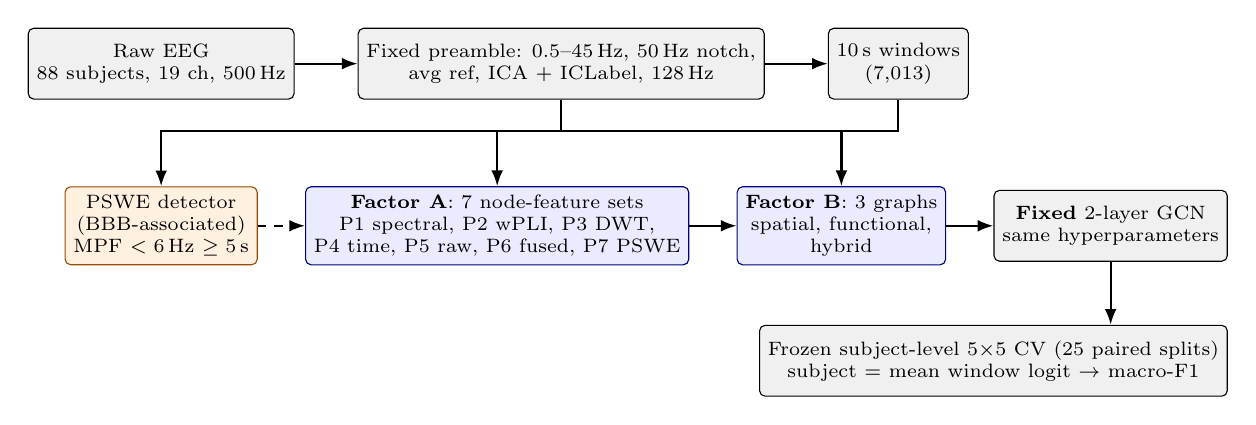
\begin{tikzpicture}[
  font=\scriptsize, node distance=5mm and 5mm,
  box/.style={draw, rounded corners=2pt, align=center, inner sep=3pt, minimum height=9mm},
  fixed/.style={box, fill=gray!12},
  vary/.style={box, fill=blue!8, draw=blue!50!black},
  bbb/.style={box, fill=orange!12, draw=orange!60!black},
  arr/.style={-{Latex[length=2mm]}, thick}]
% row 1: shared preamble
\node[fixed] (raw) {Raw EEG\\88 subjects, 19 ch, 500\,Hz};
\node[fixed, right=8mm of raw] (pre) {Fixed preamble: 0.5--45\,Hz, 50\,Hz notch,\\avg ref, ICA + ICLabel, 128\,Hz};
\node[fixed, right=8mm of pre] (win) {10\,s windows\\(7{,}013)};
% row 2: the two varied factors, the PSWE branch and the fixed model
\node[bbb, below=11mm of raw] (pswe) {PSWE detector\\(BBB-associated)\\MPF $<6$\,Hz $\ge5$\,s};
\node[vary, right=6mm of pswe] (A) {\textbf{Factor A}: 7 node-feature sets\\P1 spectral, P2 wPLI, P3 DWT,\\P4 time, P5 raw, P6 fused, P7 PSWE};
\node[vary, right=6mm of A] (B) {\textbf{Factor B}: 3 graphs\\spatial, functional,\\hybrid};
\node[fixed, right=6mm of B] (gcn) {\textbf{Fixed} 2-layer GCN\\same hyperparameters};
% row 3: evaluation
\node[fixed, below=8mm of gcn.south east, anchor=north east] (cv) {Frozen subject-level 5$\times$5 CV (25 paired splits)\\subject = mean window logit $\to$ macro-F1};
\draw[arr] (raw) -- (pre);
\draw[arr] (pre) -- (win);
\draw[arr] (pre.south) -- ++(0,-4mm) -| (pswe.north);
\draw[arr] (win.south) -- ++(0,-4mm) -| (A.north);
\draw[arr] (win.south) -- ++(0,-4mm) -| (B.north);
\draw[arr, dashed] (pswe) -- (A);
\draw[arr] (A) -- (B);
\draw[arr] (B) -- (gcn);
\draw[arr] (gcn.south) -- (gcn.south |- cv.north);
\end{tikzpicture}
\caption{Study design. Grey components are held fixed; only the node features (Factor A) and the
graph construction (Factor B) vary, in a fully crossed $7\times3$ design evaluated on the same 25
frozen subject-level splits. The PSWE detector (orange) supplies the blood--brain-barrier-associated
marker, used as P7 node features and, in an ablation, as a co-occurrence graph.}
\label{fig:pipeline}
\end{figure}


\subsection{Dataset}
We used OpenNeuro ds004504 \cite{F1,ds004504}: resting-state, eyes-closed scalp EEG from 88
participants recorded at AHEPA University Hospital (36 AD, 23 FTD, 29 cognitively normal controls,
CN). All values below were read from the dataset's own BIDS files rather than from the descriptor
paper. Recordings use 19 electrodes of the 10--20 system (Fp1, Fp2, F3, F4, C3, C4, P3, P4, O1, O2,
F7, F8, T3, T4, T5, T6, Fz, Cz, Pz) referenced to A1--A2, sampled at \SI{500}{\hertz} on a Nihon
Kohden EEG~2100 system, with a 0.4--\SI{50}{\hertz} acquisition filter. Recording length per subject
ranges from \SI{307}{} to \SI{1291}{\second} (mean \SI{802}{\second}; \SI{19.6}{\hour} in total).
Group demographics are given in Table~\ref{tab:demographics}. The data are released under CC0; the
study uses only de-identified public data. The dataset's own metadata cite a version-1.0.9 DOI that
did not resolve when checked; we cite version 1.0.8, whose EEG data are identical (the 1.0.9
changelog records only a README edit).

\begin{table}[t]
\centering\small
\caption{Participant characteristics (mean $\pm$ SD), from \texttt{participants.tsv}. MMSE is
reported for description only and is never a model input.}
\label{tab:demographics}
\begin{tabular}{lccc}
\toprule
 & AD ($n=36$) & FTD ($n=23$) & CN ($n=29$) \\
\midrule
Age (years) & $66.4\pm7.9$ & $63.7\pm8.2$ & $67.9\pm5.4$ \\
Sex (F/M) & 24/12 & 9/14 & 11/18 \\
MMSE & $17.8\pm4.5$ & $22.2\pm2.6$ & $30.0\pm0.0$ \\
\bottomrule
\end{tabular}
\end{table}

\subsection{Fixed preprocessing}\label{sec:preproc}
Every condition shares one code path, implemented with MNE-Python \cite{mne}. Raw recordings were
band-pass filtered at 0.5--\SI{45}{\hertz}, notch filtered at \SI{50}{\hertz}, and re-referenced to
the common average. Independent component analysis (extended Infomax \cite{infomax}, 18 components
--- one fewer than the channel count because of the average reference) was fitted on a
\SI{1}{\hertz} high-passed copy of each recording, and components that ICLabel \cite{iclabel}
assigned to eye or muscle artefact with probability $\ge 0.8$ were removed. Data were then resampled
to \SI{128}{\hertz} and cut into non-overlapping \SI{10}{\second} windows (1,280 samples), giving
7,013 windows in total (30--129 per subject). ICA is fitted per recording, without labels or other
subjects' data, and therefore cannot leak information across cross-validation folds; every transform
that is estimated across subjects (feature scaling, demographic residualisation) is fitted on
training subjects only.

\subsection{Factor A: node-feature representations}\label{sec:reps}
Each window is a graph whose 19 nodes are the electrodes. Seven representations define the node
features $X\in\mathbb{R}^{19\times F}$:
\begin{description}
  \item[P1, spectral ($F=7$).] Relative power in five bands (delta 0.5--4, theta 4--8, alpha 8--13,
        beta 13--30, gamma 30--45~Hz) from Welch's method \cite{welch}
        (\SI{2}{\second} Hann segments, 50\% overlap), normalised spectral entropy, and peak
        frequency within 4--15~Hz.
  \item[P2, connectivity ($F=5$).] Node strength of the weighted phase-lag index (wPLI)
        \cite{wpli,F11} in each band: the mean wPLI between a channel and the other 18.
  \item[P3, wavelet ($F=20$).] Five-level Daubechies-4 discrete wavelet transform \cite{pywavelets};
        for the sub-bands A5, D5, D4, D3 and D2 (D1, 32--\SI{64}{\hertz}, lies above the low-pass
        cut-off), relative energy, normalised coefficient entropy, mean absolute coefficient and
        standard deviation.
  \item[P4, time domain ($F=10$).] Mean, variance, root mean square, skewness, kurtosis, zero-crossing
        rate, Hjorth mobility and complexity \cite{hjorth}, sample entropy \cite{sampen} ($m=2$,
        $r=0.2\,\sigma$) and line length. Line length replaces Hjorth activity, which equals the
        variance.
  \item[P5, raw ($F=1280$).] The window z-scored per channel.
  \item[P6, fused ($F=34$).] P1, P3 and P2 concatenated, plus each node's weighted clustering
        coefficient \cite{onnela} and eigenvector centrality in the alpha-band wPLI graph.
  \item[P7, PSWE ($F=4$).] From the PSWE detector (Section~\ref{sec:pswe}): fraction of the window
        spent in a PSWE, mean and minimum median power frequency in the window, and the local PSWE
        onset rate within $\pm\SI{60}{\second}$.
\end{description}

The wPLI between channels $i$ and $j$ was computed within each window from band-passed (4th-order
Butterworth, zero-phase) analytic signals $z_i(t)$ as
\begin{equation}
  \mathrm{wPLI}_{ij} = \frac{\bigl|\langle \operatorname{Im}(z_i z_j^{*})\rangle_t\bigr|}
                            {\langle |\operatorname{Im}(z_i z_j^{*})| \rangle_t},
\end{equation}
which is insensitive to zero-lag coupling from volume conduction \cite{wpli}.

\subsection{Factor B: graph construction}\label{sec:graphs}
Three edge definitions were crossed with every representation. \emph{Spatial}: a Gaussian kernel
$w_{ij}=\exp(-d_{ij}^2/2\sigma^2)$ on Euclidean distances between standard 10--20 electrode positions,
with $\sigma$ the median pairwise distance; this graph is identical for every window and subject.
\emph{Functional}: the alpha-band wPLI of the window. \emph{Hybrid}: the element-wise product of the
two. Each graph was sparsified by keeping the $k=4$ strongest edges per node, symmetrised as
$A=\max(A,A^\top)$, kept weighted, and normalised as $\hat A = \tilde D^{-1/2}(A+I)\tilde D^{-1/2}$.

\subsection{The fixed model}\label{sec:model}
The model is the control variable, not the contribution, so a single small graph convolutional
network (GCN) \cite{F13} was used everywhere:
$H_1=\mathrm{Dropout}_{0.5}(\mathrm{BN}(\mathrm{ReLU}(\hat A X W_0)))$,
$H_2=\mathrm{ReLU}(\hat A H_1 W_1)$, mean pooling over the 19 nodes, and a linear layer to three
classes, with $W_0\in\mathbb{R}^{F\times64}$ and $W_1\in\mathbb{R}^{64\times32}$. This gives 2,819
parameters for $F=7$ and 3,651 for $F=20$; P5 is the unavoidable exception (84,355 parameters,
because $F=1280$). Two hops of propagation already reach most of a sparsified 19-node graph, and
deeper GCNs risk over-smoothing; depth is tested as an ablation. Graph attention networks
\cite{gat} learn edge weights and would partly undo the edge definitions being compared, so a GAT
is used only as a sensitivity check.

Training used AdamW (learning rate $10^{-3}$, weight decay $10^{-4}$), batch size 64, and at most
200 epochs with early stopping (patience 20) on validation macro-F1 computed at subject level. The
loss was weighted by inverse class frequency (over subjects) divided by each subject's window count,
so every subject contributes equally regardless of recording length. A subject's prediction is the
mean of its window logits. Features were standardised with statistics from training windows only.
All hyperparameters were fixed before any result was seen and are identical in every condition.

\subsection{Evaluation protocol}\label{sec:protocol}
We used subject-level, stratified, repeated 5-fold cross-validation with five repeats (seeds 0--4),
for 25 test splits of 17--18 subjects each. Within each training set, a stratified 20\% of subjects
formed the early-stopping validation set; it was never used to tune hyperparameters. The fold
assignment was generated once, verified by assertions that training, validation and test subjects
are pairwise disjoint and that every subject is tested exactly once per repeat, and committed to the
code repository before any training run. All conditions use the same 25 splits, so every comparison
is paired. The full factorial comprises $7\times3$ cells $\times$ 25 splits $=525$ training runs.

\paragraph{Confirmation folds.} Choosing the best cell, the cells to ablate and the cell to
permute on the same splits that then estimate their performance biases those estimates upwards
(the winner's curse). We therefore generated a second, independent fold assignment with the same
procedure (seeds 5--9; again 25 splits) and committed it to the repository after the main grid had
been analysed but before any run used it. The whole grid was re-run on these folds
(\nConfirmGridRuns{} runs). The cell ranked first on seeds 0--4 is reported with its score on seeds
5--9 as a selection-free estimate, and all ablations, the leakage experiment and the permutation
test reported in the main text use the confirmation folds. Their selection-fold counterparts are
given in the Supplementary material.

The primary metric is subject-level macro-averaged F1. We also report balanced accuracy, one-vs-rest
macro ROC-AUC, PR-AUC, per-class sensitivity and specificity, Cohen's $\kappa$, the Brier score,
expected calibration error and confusion matrices. Plain accuracy is reported but never used for
ranking.

\subsection{Baselines, ablations and controls}\label{sec:ablations}
\paragraph{Baselines.} A logistic regression on age and sex alone (the demographic confound floor);
a stratified random classifier (chance); and logistic regression, RBF-kernel SVM and random forest
trained on the flattened node features of each representation with the same folds, weighting and
subject aggregation as the GCN (a non-graph twin of every representation). The MMSE is never used as
an input: control participants all score 30, so it is a proxy for the label.

The GCN learns its weights from the training subjects only and uses the validation subjects only to
choose when to stop, whereas the classical models have no stopping rule. To compare models trained
on the same subjects, we evaluate both under two regimes on the same 25 test splits:
(i)~\emph{train only}, with the classical models fitted on the training subjects and the GCN as in the
main grid; and (ii)~\emph{train + val}, with the classical models fitted on training and validation
subjects and the GCN refitted on the same subjects for the number of epochs selected by early
stopping in the corresponding main-grid run (\nRefitRuns{} refits, no validation monitoring).

\paragraph{Ablations.} Run on the two best cells of the main grid, chosen automatically from the
seed 0--4 results and evaluated on the 25 confirmation splits, each paired with the same cell's
confirmation-grid run: no graph (identity adjacency, i.e.\ a per-node MLP);
degree-preserving random graphs; $k\in\{3,6\}$ and a fully connected graph; binarised edges; depth
1 and 3; GAT instead of GCN; no subject-equal weighting; demographic residualisation (age and sex
regressed out of every feature, coefficients fitted on training windows); adding P7 (PSWE) features
to the best representation; and the PSWE co-occurrence graph (Jaccard overlap of channels' PSWE
time) as the edge type.

\paragraph{Leakage.} The best cells were re-run with \emph{window-level} stratified splitting ---
windows assigned to folds at random, ignoring subject identity --- with everything else unchanged.

\paragraph{Permutation test.} For the best cell, subject labels were permuted (all windows of a
subject keep one label) and the first repeat's five folds re-run for each permutation; the
$p$-value is $(1+\#\{\text{null}\ge\text{observed}\})/(1+N)$. The primary test uses
\cpermPThreespatialN{} permutations on the first confirmation repeat (seed 5); the original
\permPThreespatialN{} permutations on the first selection repeat (seed 0) are reported for
completeness.

\subsection{PSWE detection}\label{sec:pswe}
Following Milikovsky et al.\ \cite{B1}, with parameters as reported in \cite{B3}, we computed the
median power frequency (MPF) of each channel from FFTs of \SI{2}{\second} Hann-windowed segments with
\SI{1}{\second} overlap (one MPF value per second) over 1--\SI{45}{\hertz}. The frequency range is not
reported in the source and was set to our pass-band. A PSWE is a run of at least five consecutive
seconds with MPF $<\SI{6}{\hertz}$. Detection is per channel and per recording, and uses no labels.
For each subject we computed the PSWE rate (events per minute, averaged over channels) and the
fraction of time spent in PSWEs.

\paragraph{Background-relative PSWE (exploratory).} After observing that the fixed-threshold rate
was strongly correlated with background slowing (Section~\ref{sec:res-pswe}), we added a
post-hoc analysis, labelled as such throughout. Its definitions were fixed in the configuration
before it was run on any real data. A relative PSWE is a run of at least \SI{5}{\second} in which a
channel's MPF lies below that channel's own recording-median MPF by at least \SI{2}{\hertz}
(primary), \SI{1.5}{\hertz} or \SI{3}{\hertz}, or by at least 2 or 3 robust standard deviations
($1.4826\times$ median absolute deviation).

\subsection{Statistical analysis}\label{sec:stats}
The 25 test splits are the repeated-measures units. Main effects of representation and graph
construction, and their interaction, were tested with a balanced two-way repeated-measures ANOVA on
macro-F1, reporting partial $\eta^2$ and Greenhouse--Geisser-corrected $p$-values. Because
cross-validation scores share training data and are therefore not independent, every pairwise
comparison is reported with both the Wilcoxon signed-rank test and the Nadeau--Bengio corrected
resampled $t$-test \cite{B7}, with Holm correction \cite{holm} within
each family, Cohen's $d$ and the matched-pairs rank-biserial correlation. All 21 cells were also
compared with a Friedman test and a Nemenyi critical-difference analysis \cite{demsar}. Cell-level
95\% confidence intervals come from a subject-level bootstrap (2,000 resamples of subjects within each
repeat) and from a $t$-interval over the 25 splits. The Nadeau--Bengio correction uses the ratio of
test to training subjects of the models being compared: $17.6/56.3$ for models fitted on the training
subjects only (the main grid and the ablations) and $17.6/70.4$ when validation subjects are added
(the train + val regime).

For PSWEs, group differences were tested with Kruskal--Wallis and Dunn post-hoc tests (Holm-corrected,
with rank-biserial effect sizes), and with negative-binomial regression of event counts using
recording length as exposure, adjusted for age and sex and, in further models, for relative
delta+theta power and background MPF. The relation to slowing was assessed with Spearman and
partial (age- and sex-adjusted) rank correlations, and the relation to cognition with Spearman
correlation against MMSE within patients only. All analyses were run with SciPy, statsmodels and
custom code that is tested against reference implementations.

\subsection{Compute}
All experiments ran on free Kaggle CPU sessions (4 vCPUs); no GPU was used. The 525-run main grid
took \cpuHoursGrid{} CPU-hours, and the \nConfirmRuns{} further runs (confirmation grid, ablations and permutations on the
confirmation folds, and the train + val refits) took \cpuHoursConfirm{} CPU-hours. Every run is logged with its configuration hash, code version and seed.

\section{Results}\label{sec:results}

\subsection{Data quality and the confound floor}\label{sec:res-qc}
The fixed preprocessing produced \nWindows{} windows from all 88 subjects (Figure~\ref{fig:cohort});
ICA removed on average \icaExcludedMean{} components per recording. The expected EEG slowing in
dementia was present before any model was trained: the median theta/alpha power ratio was
\thetaAlphaAD{} in AD, \thetaAlphaFTD{} in FTD and \thetaAlphaCN{} in controls, with the posterior alpha
of controls replaced by diffuse delta and theta in AD (Figure~\ref{fig:topo}).

\begin{figure}[t]
\centering
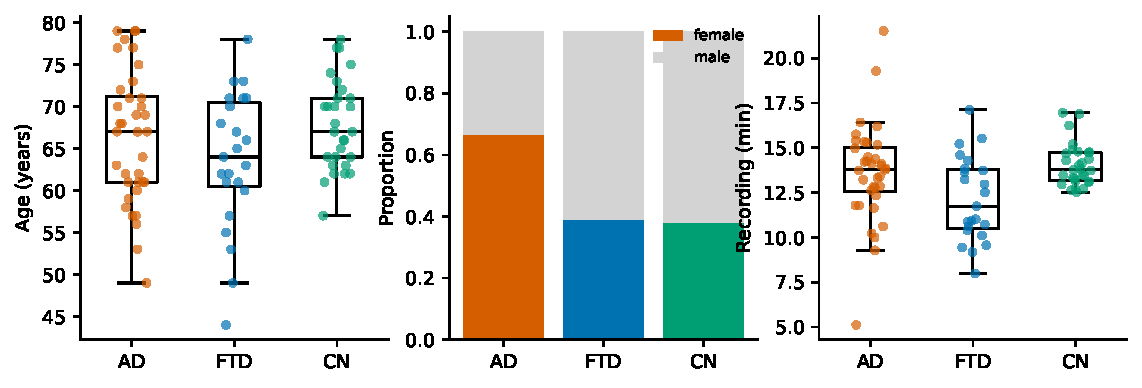
\includegraphics[width=0.9\linewidth]{fig02_cohort}
\caption{Cohort: age, sex and recording length by group.}
\label{fig:cohort}
\end{figure}

\begin{figure}[t]
\centering
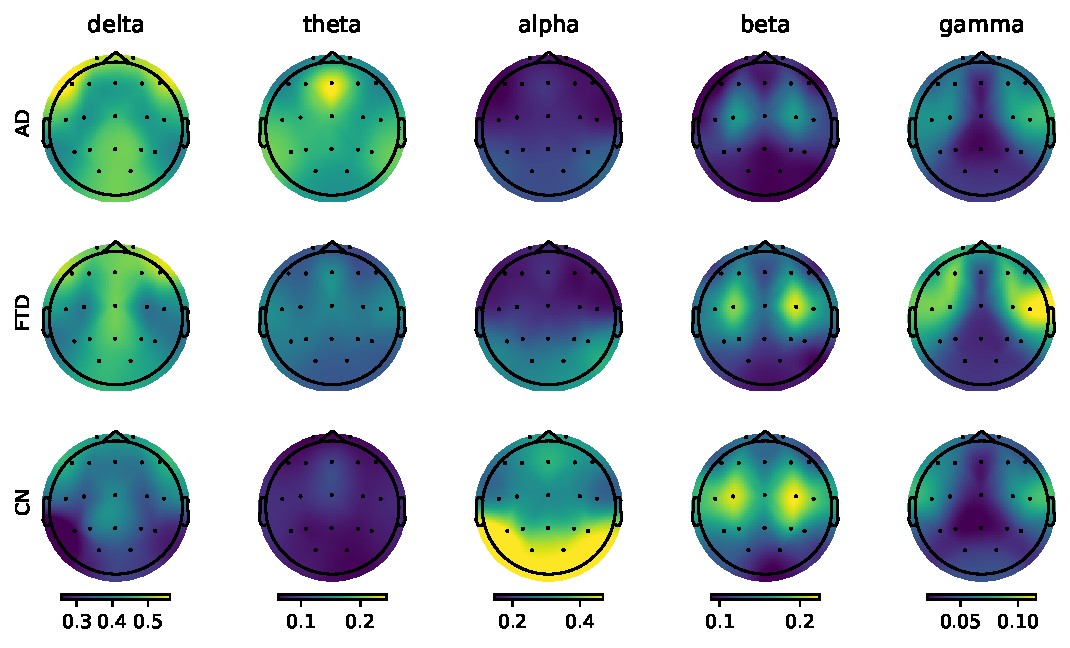
\includegraphics[width=0.9\linewidth]{fig03_band_topomaps}
\caption{Group-mean relative band power per electrode (rows: groups; columns: bands; colour scales
shared within each band).}
\label{fig:topo}
\end{figure}

A logistic regression on age and sex alone reached a macro-F1 of \demoFOne{}, against \chanceFOne{}
for a stratified random classifier. Demographics therefore carry some group information, consistent
with the sex imbalance between groups (Table~\ref{tab:demographics}). We use \demoFOne{}, not 1/3, as
the floor that EEG-based models must clear.

\subsection{Representation matters; graph construction does not}\label{sec:res-grid}
Across the 21 cells on the selection folds (\nMainRuns{} runs; Table~\ref{tab:cells}), the best
configuration was \bestCell{}, with subject-level macro-F1 \bestFOne{}~$\pm$~\bestFOneSd{}
(subject-bootstrap 95\% CI \bestFOneCiLo{}--\bestFOneCiHi{}). Because this cell was chosen as the
maximum of 21, that figure is optimistically biased. Re-evaluated on the independent confirmation
folds, the same cell scored \confFOne{}~$\pm$~\confFOneSd{} (95\% CI \confFOneCiLo{}--\confFOneCiHi{};
balanced accuracy \confBalAcc{}, macro ROC-AUC \confAuc{}, Cohen's $\kappa$ \confKappa{}) and again
ranked first of 21. The ordering of all cells was largely preserved (Spearman $\rho=\confRankRho$
between the two fold sets; Figure~\ref{fig:confirm}). We therefore take \confFOne{} as the
selection-free estimate for the best configuration.

Representation had a large effect on both fold sets (Table~\ref{tab:anova}; selection:
$F(\anovaRepDfOne,\anovaRepDfTwo)=\anovaRepF$, Greenhouse--Geisser $p\anovaRepP$, partial
$\eta^2=\anovaRepEta$; confirmation: $F=\canovaRepF$, $p\canovaRepP$, $\eta^2=\canovaRepEta$).
Averaged over graph types, the wavelet (P3, \repPThree{}; confirmation \crepPThree{}), spectral
(P1, \repPOne{}; \crepPOne{}) and fused (P6, \repPSix{}; \crepPSix{}) representations formed a leading
group; raw windows (P5, \repPFive{}) were intermediate; and connectivity strength (P2, \repPTwo{}),
PSWE features (P7, \repPSeven{}) and time-domain statistics (P4, \repPFour{}) trailed
(Figure~\ref{fig:rep}). Graph construction had a small effect on the selection folds
($F(\anovaEdgeDfOne,\anovaEdgeDfTwo)=\anovaEdgeF$, $p\anovaEdgeP$, partial $\eta^2=\anovaEdgeEta$;
marginal macro-F1 \edgespatial{} spatial, \edgefunctional{} functional, \edgehybrid{} hybrid;
Figure~\ref{fig:edge}) that did not replicate on the confirmation folds ($F=\canovaEdgeF$,
$p\canovaEdgeP$; marginal means \cedgespatial{}, \cedgefunctional{} and \cedgehybrid{}). The
representation~$\times$~graph interaction was not significant on either
(selection $F(\anovaInterDfOne,\anovaInterDfTwo)=\anovaInterF$, $p\anovaInterP$; confirmation
$F=\canovaInterF$, $p\canovaInterP$; Figure~\ref{fig:interaction}). A Friedman test across all cells
was significant ($p\friedmanP$), but the Nemenyi critical difference (\cdValue{} ranks) left the top
cells statistically indistinguishable from one another (Figure~\ref{fig:cd}).

Pairwise comparisons depend on how the dependence between cross-validation splits is handled. With
Holm-corrected Wilcoxon tests, \nPairsWilcoxonSig{} of the \nPairs{} representation pairs differed on
the selection folds and \cPairsWilcoxonSig{} on the confirmation folds; with the more conservative
Nadeau--Bengio corrected $t$-test, \nPairsNbSig{} and \cPairsNbSig{} did. For example, P3 exceeded P4
by \pThreeFourDiff{} macro-F1 on the selection folds (Cohen's $d=\pThreeFourD$; Wilcoxon--Holm
$p\pThreeFourWilP$; Nadeau--Bengio--Holm $p\pThreeFourNbP$). We regard the omnibus effect and the
ordering, which replicated, as robust, and individual pairwise differences as suggestive.

\begin{table}[t]
\centering\scriptsize
\caption{Subject-level performance of every cell (mean $\pm$ SD over the 25 selection splits,
seeds 0--4). CI: subject-bootstrap 95\% interval of macro-F1. BA: balanced accuracy; AUC: one-vs-rest
macro ROC-AUC. Confirm.: macro-F1 of the same cell on the 25 independent confirmation splits
(seeds 5--9).}
\label{tab:cells}
\setlength{\tabcolsep}{3.5pt}
\begin{tabular}{llccccccc}
\toprule
Representation & Graph & Macro-F1 & 95\% CI & BA & AUC & $\kappa$ & Brier & Confirm. \\
\midrule
\inputtab{generated/tab/cells.tex}
\bottomrule
\end{tabular}
\end{table}

\begin{table}[t]
\centering\small
\caption{Two-way repeated-measures ANOVA on subject-level macro-F1 (units: 25 test splits), on the
selection folds and, independently, on the confirmation folds. $\varepsilon$: Greenhouse--Geisser;
$p$: GG-corrected; $\eta^2_p$: partial eta squared.}
\label{tab:anova}
\setlength{\tabcolsep}{4pt}
\begin{tabular}{lccccccccc}
\toprule
 & & \multicolumn{4}{c}{Selection (seeds 0--4)} & \multicolumn{4}{c}{Confirmation (seeds 5--9)} \\
\cmidrule(lr){3-6}\cmidrule(lr){7-10}
Effect & df & $F$ & $\varepsilon$ & $p$ & $\eta^2_p$ & $F$ & $\varepsilon$ & $p$ & $\eta^2_p$ \\
\midrule
\inputtab{generated/tab/anova.tex}
\bottomrule
\end{tabular}
\end{table}

\begin{figure}[t]
\centering
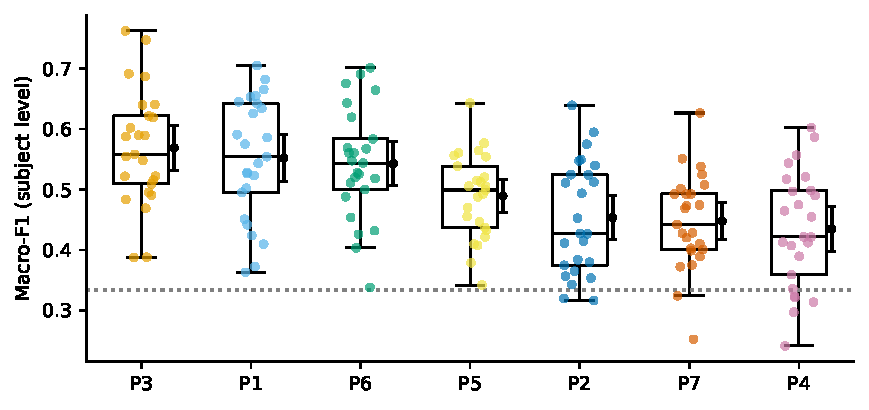
\includegraphics[width=0.62\linewidth]{fig06_representation}\hfill
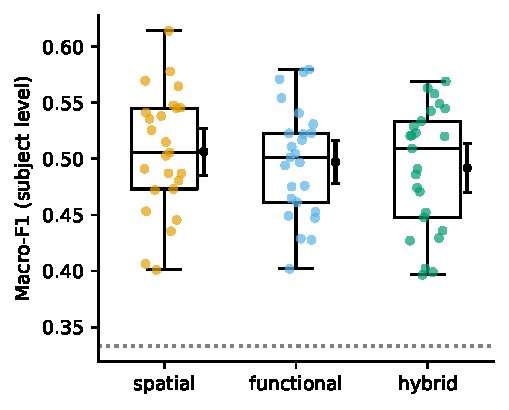
\includegraphics[width=0.33\linewidth]{fig07_edge}
\caption{Subject-level macro-F1 by representation (left, averaged over graph types) and by graph
construction (right, averaged over representations). Points are the 25 test splits; black markers,
mean $\pm$ 95\% CI; dotted line, 1/3.}
\label{fig:rep}\label{fig:edge}
\end{figure}

\begin{figure}[t]
\centering
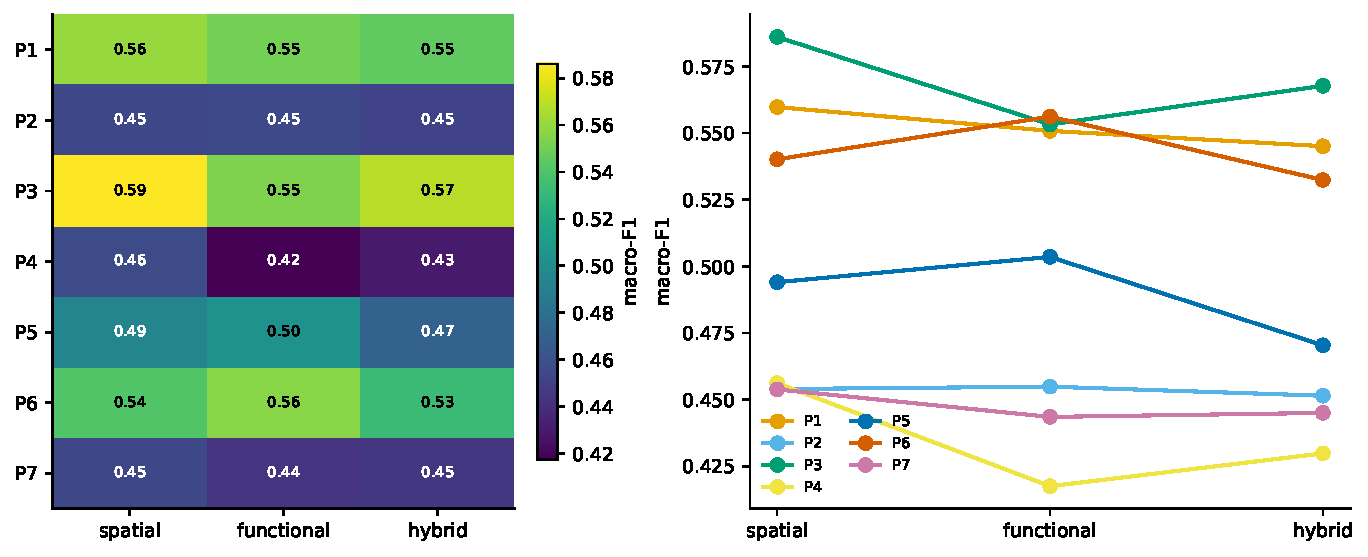
\includegraphics[width=\linewidth]{fig08_interaction}
\caption{Mean macro-F1 of every representation~$\times$~graph cell (left) and the same values as an
interaction plot (right). Lines are close to parallel: the best representation does not depend on
how the graph is built.}
\label{fig:interaction}
\end{figure}

\begin{figure}[t]
\centering
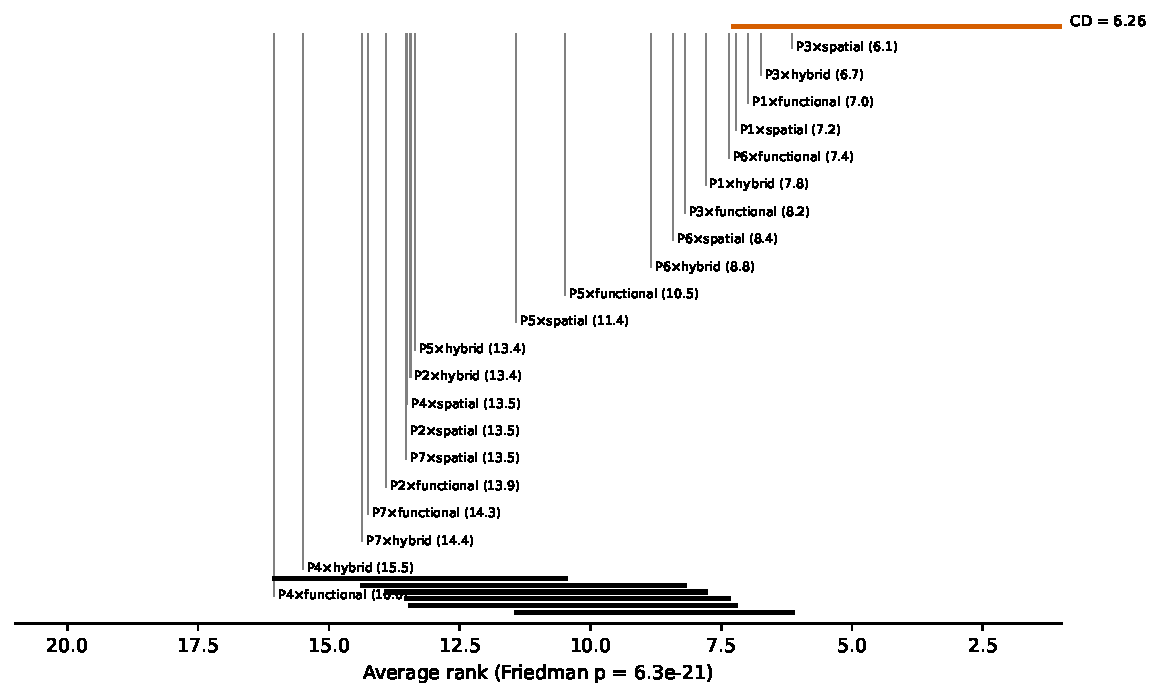
\includegraphics[width=\linewidth]{fig09_critical_difference}
\caption{Critical-difference diagram over the 21 cells. Cells joined by a black bar are not separated
by the Nemenyi test.}
\label{fig:cd}
\end{figure}

\subsection{What the models get right and wrong}\label{sec:res-errors}
For \bestCell{}, sensitivity was \bestSensCN{} for controls, \bestSensAD{} for AD and only
\bestSensFTD{} for FTD (specificities \bestSpecCN{}, \bestSpecAD{} and \bestSpecFTD{}). Across
representations, controls were recognised best and FTD --- the smallest group --- worst; FTD
recordings were most often misclassified as AD, except with PSWE features, where they were more
often taken for controls (Figure~\ref{fig:confusion}). The ROC and precision--recall
curves show the same ordering (Figure~\ref{fig:roc}). The models were poorly calibrated (expected
calibration error \bestEce{}), so their probabilities should not be read as clinical risks.

\begin{figure}[t]
\centering
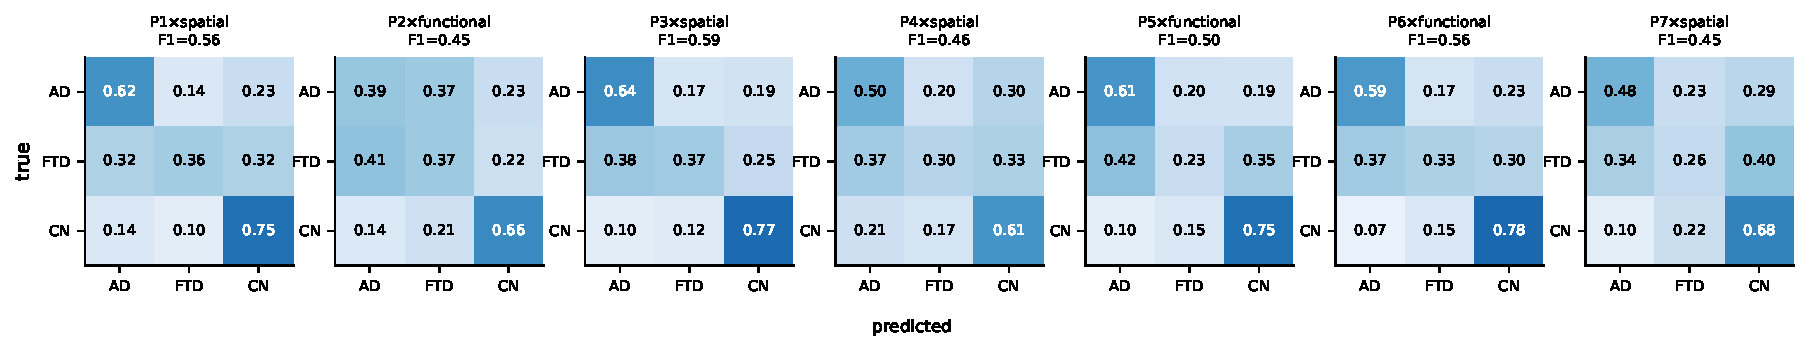
\includegraphics[width=\linewidth]{fig10_confusion_matrices}
\caption{Row-normalised confusion matrices summed over the 25 test splits, for the best graph type
of each representation.}
\label{fig:confusion}
\end{figure}

\begin{figure}[t]
\centering
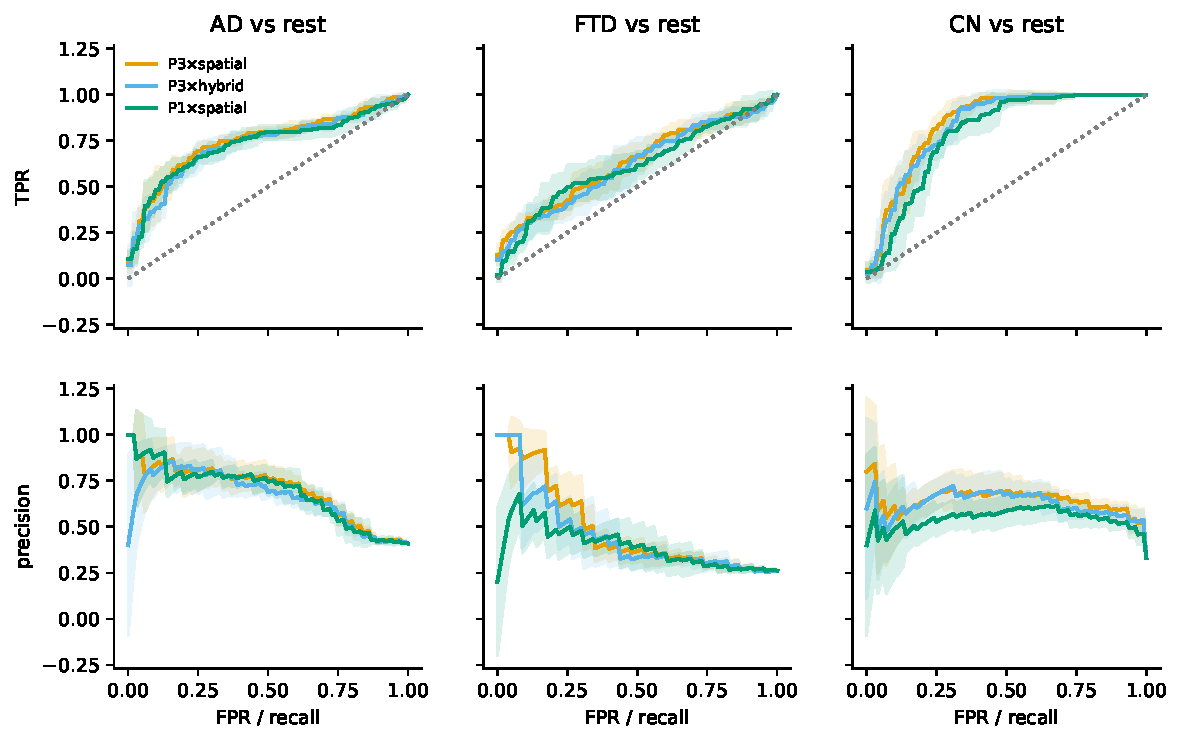
\includegraphics[width=\linewidth]{fig11_roc_pr}
\caption{One-vs-rest ROC (top) and precision--recall (bottom) curves for the three best cells; mean
$\pm$ SD across the five repeats.}
\label{fig:roc}
\end{figure}

\subsection{Graph models do not beat their non-graph twins}\label{sec:res-baselines}
Table~\ref{tab:baselines} compares every representation's best GCN cell with classical classifiers
trained on the same features, test splits and weighting, under both training regimes. With training
subjects only, the best classical model reached \classicalTrBest{}; adding the validation subjects
raised it to \classicalTvBest{}, and refitting the GCN on the same subjects raised \bestCell{} to
\refitBestFOne{} (mean gain over all cells \refitMeanGain{}). The paired difference between each
representation's best GCN cell and its best non-graph twin ranged from \fairTrDeltaMin{} to
\fairTrDeltaMax{} in the train-only regime and from \fairTvDeltaMin{} to \fairTvDeltaMax{} in the
train + val regime, and none was significant under either Holm-corrected test (Table~\ref{tab:fair};
for P3, train only: \fairTrPThreeDelta{}, Wilcoxon--Holm $p\fairTrPThreeWilP$; train + val:
\fairTvPThreeDelta{}, $p\fairTvPThreeWilP$). The GCN on wavelet features was numerically the best
model in both regimes, but its advantage over non-graph classifiers is within the noise of this
cohort. The spectral, wavelet, fused and raw representations cleared the demographic floor of
\demoFOne{}; the connectivity (P2), time-domain (P4) and PSWE (P7) representations scored within
about 0.05 of it.

\begin{table}[t]
\centering\small
\caption{Every representation's best GCN cell against its non-graph twins (same test splits,
weighting and subject aggregation) under both training regimes, and the demographic floor.
Macro-F1, mean $\pm$ SD over the 25 selection splits. Train only: models fitted on the training
subjects (the GCN early-stopped on the validation subjects). Train + val: models fitted on training
and validation subjects (the GCN refitted for its early-stopped epoch count). GCN graph type: best
in each regime.}
\label{tab:baselines}
\begin{tabular}{llcc}
\toprule
Representation & Model & Train only & Train + val \\
\midrule
\inputtab{generated/tab/baselines.tex}
\bottomrule
\end{tabular}
\end{table}

\subsection{Ablations}\label{sec:res-ablations}
Table~\ref{tab:ablations} and Figure~\ref{fig:forest} report each ablation on the confirmation folds
as a paired difference from the same cell's confirmation-grid run. No ablation reached significance
under either Holm-corrected test (\cablNSigWil{} of 26 with Wilcoxon, \cablNSigNb{} with
Nadeau--Bengio), and every point estimate except one was negative or zero: no modification improved
on the reference configuration. Removing the graph altogether (identity adjacency) changed
macro-F1 by \cablPThreespatialAOnenographDelta{} [\cablPThreespatialAOnenographLo{},
\cablPThreespatialAOnenographHi{}] for the spatial cell and by \cablPThreehybridAOnenographDelta{}
for the hybrid cell, and a degree-preserving random graph by \cablPThreespatialATworandomgraphDelta{}
and \cablPThreehybridATworandomgraphDelta{}. Any benefit of message passing is therefore small, and
we cannot attribute it to a specific electrode topology rather than to smoothing over neighbours.
Two changes had uncorrected $t$-intervals that excluded zero for the spatial cell: GAT attention
(\cablPThreespatialASixgatDelta{} [\cablPThreespatialASixgatLo{}, \cablPThreespatialASixgatHi{}]) and a
fully connected graph (\cablPThreespatialAThreefullDelta{} [\cablPThreespatialAThreefullLo{},
\cablPThreespatialAThreefullHi{}]), the latter consistent with over-smoothing; neither interval
accounts for the overlap between cross-validation training sets. Sparsity ($k=3$ or 6), binarised
edges, depth and loss weighting changed macro-F1 by at most about 0.02. Regressing age and sex out of
every feature cost \cablPThreespatialAOneTworesidualizedDelta{} [\cablPThreespatialAOneTworesidualizedLo{},
\cablPThreespatialAOneTworesidualizedHi{}] for the spatial cell, leaving performance well above the
demographic floor. The selection-fold ablations (Table~\ref{tab:ablations-main}) gave the same
conclusions.

\begin{table}[t]
\centering\scriptsize
\caption{Ablations on the confirmation folds: paired $\Delta$ macro-F1 (ablated minus the same
cell's confirmation-grid run) with 95\% $t$-interval over the 25 splits, and Nadeau--Bengio $p$ with
Holm correction within each cell. Selection-fold values: Table~\ref{tab:ablations-main}.}
\label{tab:ablations}
\begin{tabular}{lcccc}
\toprule
 & \multicolumn{2}{c}{P3 $\times$ spatial} & \multicolumn{2}{c}{P3 $\times$ hybrid} \\
\cmidrule(lr){2-3}\cmidrule(lr){4-5}
Ablation & $\Delta$ [95\% CI] & $p_\mathrm{Holm}$ & $\Delta$ [95\% CI] & $p_\mathrm{Holm}$ \\
\midrule
\inputtab{generated/tab/ablations.tex}
\bottomrule
\end{tabular}
\end{table}

\begin{figure}[t]
\centering
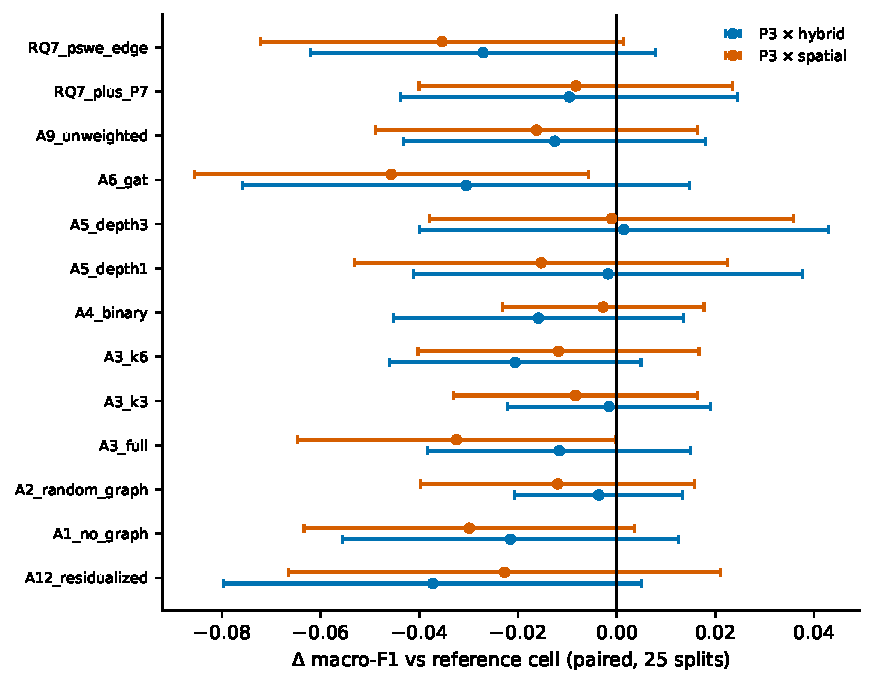
\includegraphics[width=0.75\linewidth]{fig13_ablation_forest}
\caption{Ablations on the confirmation folds as paired differences from the two reference cells
(mean and 95\% CI over 25 splits). An asterisk would mark Nadeau--Bengio--Holm $p<0.05$; none qualifies.}
\label{fig:forest}
\end{figure}

\subsection{Leakage inflates results to the published range}\label{sec:res-leak}
Re-running the two best cells on the confirmation folds with window-level splitting --- identical
data, features, graph, model and hyperparameters --- raised subject-level macro-F1 from
\cleakPThreespatialCorrectSubj{} to \cleakPThreespatialLeakySubj{} (spatial) and from
\cleakPThreehybridCorrectSubj{} to \cleakPThreehybridLeakySubj{} (hybrid). Window-level macro-F1, the
metric most often reported, rose to \cleakPThreespatialLeakyWin{} and \cleakPThreehybridLeakyWin{}
(Figure~\ref{fig:leak}). The selection folds gave almost identical values (\leakPThreespatialCorrectSubj{}
to \leakPThreespatialLeakySubj{} for the spatial cell). The leaky protocol thus reproduces the
95--99\% figures reported on this benchmark with a model that, evaluated correctly, scores about 0.6.

\begin{figure}[t]
\centering
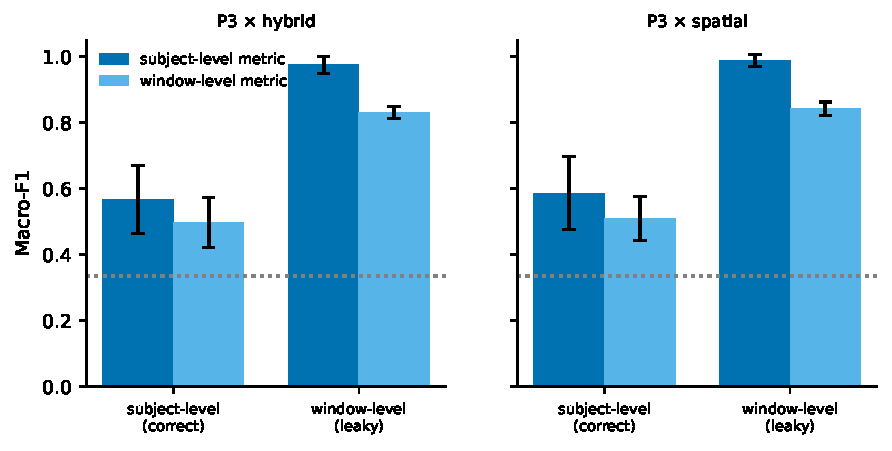
\includegraphics[width=0.8\linewidth]{fig12_leakage}
\caption{The same pipeline evaluated with subject-level (correct) and window-level (leaky)
splitting on the confirmation folds. Bars: mean $\pm$ SD over 25 splits; dotted line, 1/3.}
\label{fig:leak}
\end{figure}

\subsection{The best cell is above chance}\label{sec:res-perm}
On the first confirmation repeat, the observed macro-F1 of \bestCell{} was \cpermPThreespatialObs{},
against a label-permutation null with mean \cpermPThreespatialNullMean{} and maximum
\cpermPThreespatialNullMax{} over \cpermPThreespatialN{} permutations ($p=\cpermPThreespatialP$, the
smallest value attainable; Figure~\ref{fig:perm}). The original test on the selection folds gave the
same result (\permPThreespatialN{} permutations, observed \permPThreespatialObs{}, null maximum
\permPThreespatialNullMax{}, $p=\permPThreespatialP$).

\subsection{PSWE: a BBB-associated marker that tracks slowing}\label{sec:res-pswe}
Fixed-threshold PSWEs were most frequent in AD (median \psweRateAD{} events/min), intermediate in FTD
(\psweRateFTD{}) and least frequent in controls (\psweRateCN{}; Kruskal--Wallis $p\psweKwP$;
Figures~\ref{fig:pswe-example} and~\ref{fig:pswe}). In negative-binomial models adjusted for age and
sex, the PSWE rate ratio relative to controls was \psweAdjADRR{} (95\% CI \psweAdjADLo{}--\psweAdjADHi{},
$p\psweAdjADP$) in AD and \psweAdjFTDRR{} (\psweAdjFTDLo{}--\psweAdjFTDHi{}, $p\psweAdjFTDP$) in FTD.

The PSWE rate was, however, almost collinear with background slowing (Spearman $\rho=\psweSlowRho$
with relative delta+theta power; age- and sex-adjusted partial $\rho=\psweSlowPartial$). Once slowing
was added to the model, the AD rate ratio reversed to \psweAdjSlowADRR{} (\psweAdjSlowADLo{}--\psweAdjSlowADHi{},
$p\psweAdjSlowADP$), and FTD fell to \psweAdjSlowFTDRR{} ($p\psweAdjSlowFTDP$). The PSWE rate was not
significantly associated with MMSE within patients ($\rho=\psweMmseRho$, $p\psweMmseP$). In the
classifier, PSWE features alone (P7) performed near the demographic floor (\repPSeven{}), and adding
them to the best representation, or using PSWE co-occurrence as the graph, did not help
(Section~\ref{sec:res-ablations}).

\paragraph{Background-relative PSWEs (exploratory).} Defining PSWEs relative to each channel's own
background reversed the group pattern. With the primary definition (a drop of at least \SI{2}{\hertz}
below the channel median), AD showed \emph{fewer} transient slowing events than controls (rate ratio
\reldropTwoAdjADRR{}, \reldropTwoAdjADLo{}--\reldropTwoAdjADHi{}, $p\reldropTwoAdjADP$), FTD a
non-significant reduction (\reldropTwoAdjFTDRR{}), and the event rate was only weakly related to
slowing ($\rho=\reldropTwoSlowRho$) and not to MMSE ($\rho=\reldropTwoMmseRho$). After additional
adjustment for background MPF the AD effect was no longer significant (\reldropTwoAdjBgADRR{},
$p\reldropTwoAdjBgADP$). The MAD-scaled variants gave the same direction more strongly and survived
that adjustment (for 2~MAD: AD \relmadTwoAdjBgADRR{}, $p\relmadTwoAdjBgADP$; FTD \relmadTwoAdjBgFTDRR{},
$p\relmadTwoAdjBgFTDP$). Every variant pointed the same way: relative to their own background,
patients with dementia had fewer, not more, transient slowing events.

\begin{figure}[t]
\centering
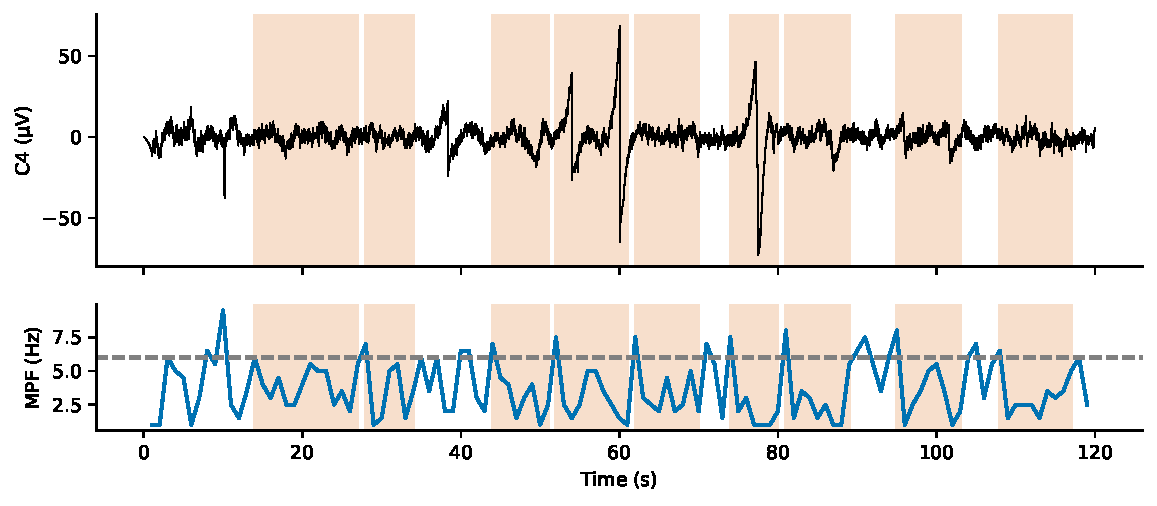
\includegraphics[width=\linewidth]{fig04_pswe_example}
\caption{Fixed-threshold PSWE detection in the AD recording with the highest PSWE rate among the
example shard (first 120\,s, channel with most events). Top: EEG; bottom: median power frequency
with the \SI{6}{\hertz} threshold; shaded, detected PSWEs. Because this subject's background is
already slow, most of the recording is flagged --- the pattern behind the collinearity with slowing.}
\label{fig:pswe-example}
\end{figure}

\begin{figure}[t]
\centering
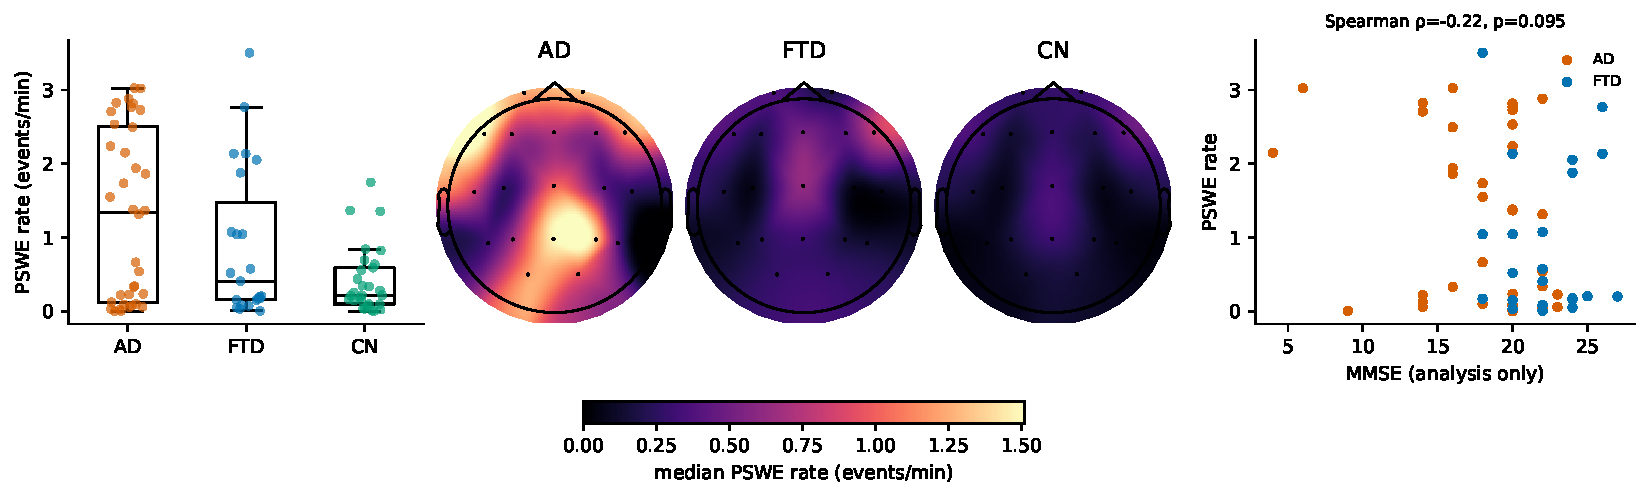
\includegraphics[width=\linewidth]{fig05_pswe_burden}
\caption{Fixed-threshold PSWE rate per subject by group (left), median per-channel rate as scalp maps
(middle), and rate against MMSE in patients (right; analysis only).}
\label{fig:pswe}
\end{figure}

\section{Discussion}\label{sec:discussion}

\subsection{Principal findings}
Holding the model, data and evaluation protocol fixed, we found four things. First, the node-feature
representation strongly affects three-class AD/FTD/control classification (partial
$\eta^2=\anovaRepEta$), with wavelet, spectral and fused features leading. Second, how the graph is
built matters little (partial $\eta^2=\anovaEdgeEta$), the best representation does not depend on it,
and the GCN performs no better than a random forest or SVM on the same features. Third, splitting
windows instead of subjects inflates subject-level macro-F1 from about 0.59 to about 0.99 on the
identical pipeline, reproducing the top of the published range. Fourth, the
blood--brain-barrier-associated PSWE marker is more frequent in AD and FTD than in controls, but this
excess is explained by continuous background slowing; defined relative to each person's background,
transient slowing events are, if anything, less frequent in dementia.

\subsection{Representation matters more than topology}
The size and consistency of the representation effect, against a small and non-interacting graph
effect, indicate that the information a GNN can use on this benchmark lives mostly in the node
features. Several observations point the same way. Spatial graphs --- which are identical for every
subject and therefore carry no diagnostic information of their own --- did at least as well as
functional and hybrid graphs. A degree-preserving random graph cost about as much as removing the
graph altogether, which suggests that message passing helps, where it helps at all, by smoothing
features over neighbouring electrodes rather than by exploiting a particular connectivity pattern.
And non-graph classifiers on flattened features matched the GCN cell for cell. These results agree
with the independent conclusion of the 2026 scoping review that apparent representational gains on
this dataset do not survive leakage-free evaluation \cite{R1}, and they temper the case for
graph-based modelling made in recent work \cite{R2,R8,F7}: on 19-electrode scalp EEG from 88
subjects, we see no evidence that graph structure adds information beyond good node features. Whether
this holds with source-space nodes, learned adjacency or much larger cohorts remains open.

\subsection{Neurophysiological interpretation}
Representations that describe each electrode's own spectrum (P1, P3) outperformed one built only from
inter-electrode phase coupling (P2), and the functional graph did not improve on the spatial one.
Within the limits of scalp EEG, this favours local oscillatory slowing over altered large-scale
coupling as the dominant discriminative signal, consistent with spectral slowing being the most
replicated EEG marker of AD \cite{R3,R15} and with the posterior-alpha-to-diffuse-theta shift visible
in our data (Figure~\ref{fig:topo}). It does not contradict network accounts of dementia
\cite{F12,F9}: alpha-band wPLI estimated within \SI{10}{\second} windows is noisy, and electrode-level
graphs are a coarse proxy for cortical networks. The error pattern is clinically recognisable:
controls are identified best, while FTD --- the smallest group, and less slowed than AD --- is
identified worst and is usually mistaken for AD. Separating the two dementias remains the hard part of the problem.

\subsection{What the PSWE results mean for an EEG marker of BBB dysfunction}
With the fixed threshold, our data agree in direction with Milikovsky et al.: PSWE rates were roughly
three times higher in AD than in controls after adjusting for age and sex, and FTD --- not previously
studied --- was also elevated. Two further analyses change the interpretation. The fixed-threshold
rate was almost collinear with relative delta+theta power, and adjusting for that slowing reversed
the AD effect. When events were instead defined as transient drops below each channel's own
background, AD and FTD showed fewer of them than controls, under every variant we examined. Together
these results suggest that, in resting scalp EEG with diffuse slowing, a median power frequency below
\SI{6}{\hertz} mostly flags a slow \emph{background} rather than \emph{paroxysmal} events.

We draw three cautious conclusions. First, a fixed-threshold PSWE rate should not be read as evidence
of BBB dysfunction without controlling for background slowing. Second, background-relative
definitions are needed if PSWEs are to capture transient cortical dysfunction, although they bring
their own floor effect in very slow recordings, which we observed in the Hz-drop variants. Third, our
data cannot test the BBB link itself: ds004504 contains no BBB imaging, the original detection
details include parameters we could not verify from the full text, and Milikovsky et al.\ studied
different patients under different recording conditions. The decisive test is a cohort with both EEG
and dynamic contrast-enhanced MRI.

\subsection{Implications for how results on this benchmark are read}
On one pipeline, the choice between subject-level and window-level splitting moved subject-level
macro-F1 by about 0.4 --- roughly three times the gap between the best and worst representation, and
several times larger than any graph or architecture change we tested. Figures in the high 90s on ds004504 should therefore be read alongside their
splitting protocol, and studies that report window-level metrics or allow a subject's windows into
both training and test sets cannot be compared with subject-level results. We name no individual
study: the point is that the protocol, not the model, determines most of the reported number, as
argued independently in \cite{R1,F8}. The permutation test confirms that the honest result is
nonetheless real.

\subsection{Limitations}
The cohort is small: test folds contain 17--18 subjects, and under the conservative Nadeau--Bengio
correction no pairwise difference between representations, and no single ablation, reached
significance. We report both corrected and uncorrected tests and give effect sizes, but small
differences between leading representations should not be over-interpreted. All data come from one
site, device and protocol, and FTD is the smallest class ($n=23$). The planned external validation on
an independent cohort (ds004584) and two planned ablations (window length and ICA on/off) were not
run for this draft. Hyperparameters were fixed a priori and not tuned; early stopping on a
validation set of about 14 subjects stopped training early, which may disadvantage higher-capacity
configurations such as raw windows (P5, about 84k parameters). Calibration was poor. Graphs are
defined on electrodes rather than cortical sources. The demographic floor (\demoFOne) shows residual
age and sex information, which residualisation reduced but did not remove. For PSWEs, the MPF
frequency range was not reported in the source and was set by us, we detected events per channel
rather than over averaged regions, the background-relative analysis is post hoc, and no BBB measure
is available.

\subsection{Future work}
The most valuable next study is a multi-site replication of this exact protocol, since a single-site
design cannot establish device or population invariance. Natural extensions are source-space graphs
\cite{F7}, learned adjacency \cite{F4}, spatio-temporal graphs over window sequences \cite{R10,F6},
an architecture sweep under a fixed representation (the transpose of this design) \cite{F5}, an
MCI class, and --- for the BBB question --- simultaneous EEG and dynamic contrast-enhanced MRI to test
whether any PSWE definition tracks measured barrier leakage \cite{B5,B8}.

\section{Conclusion}\label{sec:conclusion}
We asked whether the performance of graph neural networks for EEG-based dementia classification comes
from how the signal is represented, how the brain graph is built, or the model. On a public
88-subject benchmark, with the model, data and evaluation protocol held fixed and seven
representations crossed with three graph constructions over 25 paired subject-level splits, the
answer is mostly the representation: wavelet and spectral node features lead, graph construction
matters little, and the GCN does not outperform non-graph classifiers on the same features. The best
honest three-class macro-F1 was \bestFOne{}, clearly above chance ($p=\permPThreespatialP$) but far
below published figures --- a gap that window-level splitting alone closes on our own pipeline,
inflating subject-level macro-F1 to \leakPThreespatialLeakySubj{}. A blood--brain-barrier-associated
EEG marker, the paroxysmal slow-wave event, was elevated in AD and FTD under its original definition
but was explained by background slowing, and defining it relative to each person's background
reversed the effect. We release the code, seeds, frozen folds and every raw run so that each number
in this paper can be regenerated from the data.


\section*{Data and code availability}
The EEG data are OpenNeuro ds004504 (CC0) \cite{ds004504}. Code, configuration
(\texttt{configs/default.yaml}), the frozen fold assignment (\texttt{splits/folds\_ds004504.json},
with the SHA-256 of \texttt{participants.tsv}), every raw training run (one JSON record per run,
with configuration hash, code version, seed and per-subject test predictions), and the Kaggle
notebooks that produced them are available at
\url{https://github.com/Devguru-codes/Major_project_IIITN}. Random seeds are 0--4 for the main grid
and ablations, and $10{,}000+i$ for permutation $i$. Every table and figure in this paper is
regenerated from the committed raw runs by a single command (\texttt{python -m eegrep report}), and
the resolved package versions are recorded in \texttt{reports/kaggle\_pip\_freeze.txt}. The full study
runs on free cloud CPUs.


\bibliographystyle{unsrtnat}
\bibliography{references}

\clearpage
\appendix
\section*{Supplementary material}
\renewcommand{\thefigure}{S\arabic{figure}}\setcounter{figure}{0}

\begin{figure}[h]
\centering
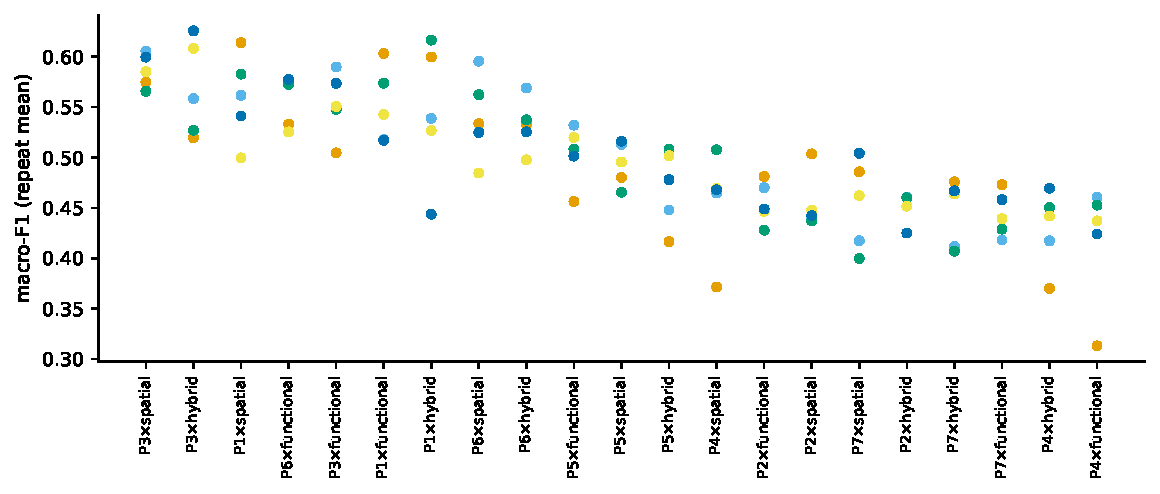
\includegraphics[width=\linewidth]{figS3_seed_variance}
\caption{Mean macro-F1 of each repeat (seed) for every cell: variation due to the cross-validation
partition and initialisation.}
\label{fig:seeds}
\end{figure}

\begin{figure}[h]
\centering
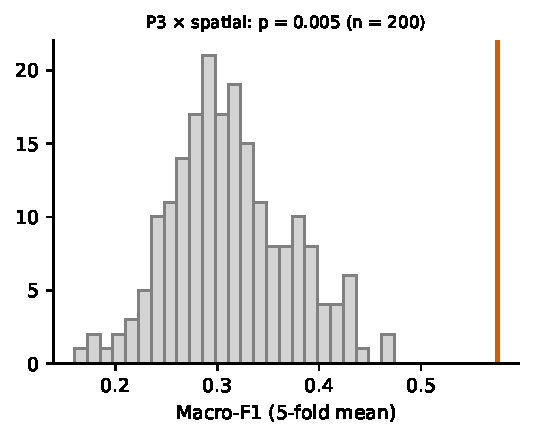
\includegraphics[width=0.5\linewidth]{figS5_permutation_null}
\caption{Label-permutation null distribution (200 permutations, first repeat's five folds) for the
best cell; red line, observed macro-F1 on the same splits.}
\label{fig:perm}
\end{figure}

\end{document}
